\documentclass[english]{scrartcl}

\usepackage{fullpage}
\usepackage{amstext,amssymb,amsmath,amsthm}
\usepackage{graphicx,subfigure}
\usepackage{multirow}
\usepackage{url}
\usepackage{hyperref}
\usepackage{color}

\graphicspath{{.}{pics/}}

%\newtheorem{theorem}{Theorem}[section]
%\newtheorem{proposition}[theorem]{Proposition}


\title{Composite Bayesian inference}
\date{}
\author{Alexis Roche\thanks{\url{alexis.roche@centraliens.net}}}

\def\x{{\mathbf{x}}}
\def\y{{\mathbf{y}}}
\newcommand{\blambda}{{\boldsymbol{\lambda}}}
\newcommand{\bell}{{\boldsymbol{\ell}}}
\newcommand{\E}{\mathbb{E}}
%\newcommand{\matphi}{\boldsymbol{\Phi}} 
%\def\p{{\bar{\mathbf{p}}}}
%\def\q{{\bar{\mathbf{q}}}}



\begin{document}

\maketitle

\begin{abstract}
We revisit the concept of composite likelihood as a method to make a probabilistic inference by aggregation of multiple Bayesian agents. This view makes it natural to use a machine learning approach to calibrate the weights associated with composite likelihood. In a supervised learning scenario, for instance, they can be set so as to minimize training cross-entropy, yielding an easy-to-solve convex problem. We argue that composite Bayesian inference is a middle way between generative and discriminative modeling approaches that trades off between interpretability and prediction performance, both of which are crucial to many artificial intelligence tasks.
\end{abstract}


\section{Introduction}
\label{sec:intro}

Textbook statistical inference (frequentist or Bayesian) rests upon the existence of a probabilistic data-generating model that is both empirically valid and computationally tractable. Because this double requirement may be very challenging for multi-dimensional data, other inference models have been developed in applied science: deliberately misspecified generative models, as in quasi-likelihood \cite{White-82,Walker-13} or na\"ive Bayes \cite{Ng-01} methods; data compression models as in the minimum description length paradigm \cite{Grunwald-07}; and discriminative models\footnote{A {\em discriminative} model is a parametric family that describes the distribution of a target variable conditional on the data, in contrast with a {\em generative} model, which describes the conditional distribution of the data given the target variable.}, which currently dominate the field of artificial intelligence (AI) and typically require supervised learning on large datasets -- these include many classical ``shallow'' learning \cite{Ho-95,BergerA-96,Vapnik-00,Rasmussen-06} and deep learning \cite{Lecun-15,Goodfellow-16} techniques (with the exception of deep belief networks \cite{Hinton-06}).

% Retravailler cette histoire de causalite. Ce qui est dit dans ce pragaraphe est faux. N'import quel seuillgage fait apparaitre la profondeur de l'objet comme "cause" de la classification. Ce qu'un modele discriminant ne permet pas, c'est de dire si les donnees observees sont "typiques" de telle ou telle classe. 

Discriminative models, however, lack the ability to establish {\em causality} links between data instances and predictions, and therefore cannnot {\em explain} their own predictions. Consider as a straightforward example the problem of deciding whether a pan is a sauce pan or a frying pan based on its depth. A discriminative model can learn a threshold that correctly classifies most pans in practice, but it cannot gain an explicit internal representation that sauce pans tend to be deeper than frying pans, which is {\em why} the thresholding works. The only way to interpret a discriminative model is to ``reverse engineer'' it using external knowledge, which is an almost impossible task for high-dimensional models.

There is growing awareness that AI should be interpretable in life-impacting applications~\cite{Molnar-18}, where it is (and perhaps should remain) confined to a supportive role in human-driven decision making processes. For instance, in medical diagnosis, automated disease predictions should always be corroborated by individualized findings to be communicable to clinicians -- in other words, there is no interest for ``black boxes'' but for AI systems that can justify their opinions just like human experts. On the other hand, clinicians have long used reference range analysis for diagnosis, which stems from simple univariate generative models.

%, {\em e.g.}, by pinpointing biomarkers that deviate from healthy reference ranges.

% simple methods based on range analysis of univariate biomarkers can provide meaningful clues, and are thus more useful in practice although less powerful in terms of prediction performance.

%With generative models you can compare data with expected outcomes to get insight. 

%the information they provide to support them is limited to the boundaries between classes, which are difficult to interpret for high-dimensional data representations. 

%Decision making is not about pooling opinions, it is about pooling empirical observations and find which hypothesis they point to.

%Need to emphasize why we need generative models. Below are some valid reasons: unsupervised learning, potentially better performance on small training datasets... But the \#1 reason is that discriminative models are black boxes: they provide an answer but no explanation to support it. Truth is, they perform better in supervised big data context in the sense of accuracy, cross-entropy, and so on, no question about that -- but they are mere inference recipes. Is that what AI should be? Sometimes, yes. But there are application fields where this clearly cannot work, for instance medical diagnosis. 

%Imagine a doctor telling a patient: ``Sorry, sir, you have Alzheimer's disease because this fancy AI software said so''. Unless the said software is 100\% reliable, which is practically impossible, this would obviously be unacceptable. Acceptable would be to corroborate the diagnosis with some key quantitative empirical observations: low memory test scores, hippocampal atrophy, etc. In other words, inference has to come with some insight. An AI system is but one expert relying on hypotheses which may be invalid, as any expert, and is therefore prone to error. A typical error source is to train a classifier on a subset of classes from the real world. We cannot avoid inference errors but we can safeguard against them by being able to interrogate the system: why do you think what you think? To achieve that, the system should be capable of {\em introspection.

%Vapnik: ``one should solve the classification problem directly and never solve a more general problem as an intermediate step''. True if the goal is classification only. Wrong if introspection is needed because the problem is then more general in nature.

%Human inference does not work in a pre-determined universe of ``causes''. We confront theories with reality to evaluate how likely they are, while knowing that none of the theories considered so far may be ``right''. In fact, we are not looking for the truth, but for a conving enough theory. 

%Composite likelihood seen as a pool of experts comes with a potential introspection mechanism: first sort experts by decreasing influence on the predictive distribution, see how likely the different classes are to the most influential experts.

Another limitation of discriminative models is that they are not suitable for unsupervised learning or on-the-fly parameter estimation because they treat the data and the model parameters as {\em marginally independent} variables, meaning that the data conveys no information about the parameters unless the target variable is observed. This is illustrated in Figure~\ref{fig:graph_comparison} by the respective directed graphs representing generative and discriminative models. For the same basic reason, supervised learning in a discriminative model is statistically less efficient than in a generative model spanning the same family of posteriors, hence it requires more training data to achieve optimal performance \cite{Ng-01}. 

%Overall, pure discriminative models are of little use outside the context of big labeled data.

\begin{figure}[!ht]
\begin{center}
\subfigure[Generative model]{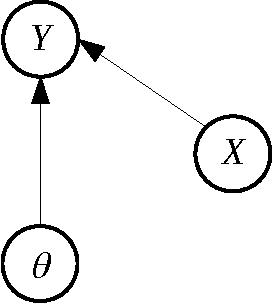
\includegraphics[width=.25\textwidth]{generative.pdf}\label{fig:generative}}
\hspace*{.2\textwidth}
\subfigure[Discriminative model]{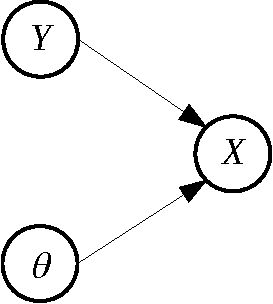
\includegraphics[width=.25\textwidth]{discriminative.pdf}\label{fig:discriminative}}
\caption{Directed graphs representing generative and discriminative models, where $X$, $Y$ and $\theta$ respectively denote the target variable, the data, and the model parameters. Note the marginal independence of data and parameters in the discriminative model.}
\label{fig:graph_comparison}
\end{center}
\end{figure}

This note advocates probabilistic opinion pooling \cite{Genest-86} as a means to incorporate generative information into a discriminative model. Rather than attempting at a full generative model, one may combine multiple low-dimensional generative models corresponding to different pieces of information extracted from the input data. Each such model acts as an isolated ``agent'' using a single feature to express an opinion in the form of a likelihood function of the target variable. The agent opinions may then be aggregated into a unique predictive probability distribution analogous to a Bayesian posterior.

This idea may be understood as a probabilistic version of boosting, or as a ``divide and conquer'' approximation to the intractable Bayesian posterior. Importantly, predictions made in such a way are interpretable owing to their underlying generative nature.

When choosing the aggregation method as a log-linear pool, the predictive distribution turns out to be proportional to a quantity known as composite likelihood (CL) in computational statistics. As detailed in \cite{Varin-11} and the references therein, CL was developed as a surrogate of traditional likelihood for parameter estimation. While maximum CL does not inherit the general property of maximum likelihood to achieve asymptotical minimum variance, it is asymptotically consistent under mild conditions \cite{Xu-11} and generally offers an excellent trade-off between computational and statistical efficiency.

With the opinion pooling interpretation in mind, the weights assigned to the different features may be optimized for prediction performance in a typical discriminative learning scenario. As we will see, this strategy amounts to training a maximum entropy classifier using the feature-based log-likelihoods as basis functions. These likelihood functions themselves may need to be pre-trained, therefore the composite inference approach typically invovles a double training scheme: a generative training stage (to learn feature-based likelihood parameters) followed by a discriminative training stage (to learn feature weights in aggregation).

Technical details are given in the remainder.



\section{Composite likelihood as opinion pooling}
\label{sec:log_pool}

Let $\mathbf{Y}$ an observable multivariate random variable with sampling distribution $p(\y|x)$ conditional on some unobserved variable of interest, $X\in{\cal X}$, where ${\cal X}$ is assumed to be a finite set for simplicity. Given an experimental outcome $\y$, the likelihood is the sampling distribution evaluated at $\y$, seen as a function of $x$:
$$
L(x) = p(\y|x)
.
$$

This requires a plausible generative model which, for complex data, may be out of reach or involve too many parameters to be estimated. A natural workaround known as data reduction is to extract some lower-dimensional representation $z=f(\y)$, where $f$ is a many-to-one mapping, and consider the potentially more convenient likelihood function:
$$
\ell(x) = p(z|x)
.
$$

Substituting $L(x)$ with $\ell(x)$ boils down to restricting the feature space, thereby  ``delegating'' statistical inference to an ``agent'' provided with partial information. While it is valid for such an agent observing~$z$ only to consider $\ell(x)$ as the likelihood function of the problem, the drawback is that $\ell(x)$ might yield too vague a prediction of~$X$ due to the information loss incurred by data reduction. To make the trick statistically more efficient, we may extract several features, $z_i=f_i(\y)$ for $i=1,2,\ldots,n$, and try to combine the likelihood functions $\ell_i(x) = p(z_i|x)$ that they elicit.

If we see the likelihoods as posterior distributions corresponding to uniform priors, this is a classical problem of probabilistic opinion aggregation from possibly redundant sources, for which several methods exist in the literature \cite{Tarantola-82,Genest-86,Garg-04,Allard-12}. One that is appealing as it tends to produce single peaked distributions is the {\em generalized logarithmic opinion pool}:
\begin{equation}
\label{eq:log_pool}
p_\blambda(x|\y) \propto \pi(x) \prod_{i=1}^n p(z_i|x)^{\lambda_i},
\end{equation} 
where $\pi(x)$ is a prior distribution, and $\blambda=(\lambda_1,\ldots,\lambda_n)$ is a vector of weights. Negative weights should be ruled out to warrant a natural monotonicity property: if all agents agree that an outcome $x_1$ is less likely than an outcome $x_2$, then the consensus probabilities should always satisfy $p_\blambda(x_1|\y)\leq p_\blambda(x_2|\y)$. Also note that it is possible to have the weights depend on the data~$y$, but this would make the method considerably more complex and less interpretable. 


%This condition holds whenever all weights are positive ($\lambda\succeq 0$), assuming that the agent opinions are upper bounded. Negative weights should be ruled out to warrant a natural monotonicity property: if all agents agree that an outcome $x_1$ is less likely than an outcome $x_2$, then the consensus probabilities should always satisfy $p_\lambda(x_1|\y)\leq p_\lambda(x_2|\y)$. Note that it is possible to have the weights depend on the data~$y$, but this would make the method considerably more complex and less interpretable. 


%Strictly positive weights guarantee the so-called 0/1 forcing property, that is, if an hypothesis~$x$ has zero likelihood according to at least one agent, then its consensus probability vanishes too.

% Not clear yet as to what a negative weight could mean!


\section{Composite Bayes rule}
\label{sec:bayes_rule}

The log-linear pool~(\ref{eq:log_pool}) bears a striking similarity to Bayes rule, yielding  the form: 
$$
p_\blambda(x|\y)\propto \pi(x) L^c_\blambda(x),
$$
where the distribution $\pi(x)$ plays the role of a prior, and the function:
\begin{equation}
\label{eq:comp_lik}
L^c_\blambda(x) \equiv \prod_{i=1}^n \ell_i (x)^{\lambda_i}
\end{equation} 
plays that of a likelihood function. The expression~(\ref{eq:comp_lik}) happens to be known in computational statistics as a {\em marginal composite likelihood} \cite{Varin-11}. The slightly more general {\em conditional composite likelihood} form can be derived in the same way as above by conditioning all probabilities on confounding variables, see Appendix~\ref{appendix:conditional}. The computational advantage of CL over a genuine likelihood function stems from the fact that it is more efficient to evaluate the marginal distributions of each feature than the joint distribution of all features.

CL shares a convenient factorized form with the likelihood derived under the assumption of mutual feature independence, usually referred to as {\em na\"ive Bayes} or {\em simple Bayes} in the machine learning literature, which corresponds to the special case of unitary weights, $\blambda\equiv 1$. While the above derivation does not assume feature independence, it yields an alternative interpretation of na\"ive Bayes as a general feature aggregation method. However, unitary CL weights do not guarantee optimal prediction performance.


\section{Prediction interpretation}

A compelling advantage of the composite approach is to make it easy to interpret a prediction for any instance~$\y$. Given two putative target values $x_0$ and $x_1$, the log-probability ratio of $x_1$ vs~$x_0$ is computed by simply adding up single-feature contributions: 
$$
\log \frac{p_\blambda(x_1|\y)}{p_\blambda(x_0|\y)}
= 
\underbrace{\log \frac{\pi(x_1)}{\pi(x_0)}}_{\text{offset}}
+ \sum_i \underbrace{\lambda_i \log \frac{p(z_i|x_1)}{p(z_i|x_0)}}_{\text{feature contribution}},
$$
therefore it is straightforward to assess which features contribute most to a particular hypothesis comparison (either positively or negatively), see possible disagreements between features, and corroborate predictive probabilities with feature-level testable information. 

Each feature contributes to an hypothesis comparison proportionally to its associated log-likelihood ratio test statistic. Contrary to statistical hypothesis testing, likelihood ratios are not converted into $p$-values but are directly combined into a predictive probability ratio. Non-unitary composite weights reinforce or inhibit features compared to na\"ive Bayes prediction ($\blambda\equiv 1$), and may therefore account for mutual feature dependence if tuned appropriately. Keeping the analogy with hypothesis testing, composite weights may be thought of as the counterpart of multiple testing correction \cite{Benjamini-10}.

To interpret the predictive distribution globally, the user(s) may go through successive pairwise hypothesis comparisons in a dynamic way, starting by comparing the automated prediction, {\em i.e.} the most probable target, to some educated guess or reference class (for instance, normality in medical diagnosis). Next, depending on the feature contributions highlighted by the comparison, they may submit another hypothesis for comparison to the automated prediction. This process may be repeated until the composite prediction is subjectively understood by the user(s), yielding a form of human machine dialog.



\section{Composite weight tuning}
\label{sec:tuning}

%So far, we have assumed that the composite weights~$\blambda=(\lambda_1,\ldots,\lambda_n)$ in~(\ref{eq:log_pool}) are known. 

Let us now turn to the problem of tuning the composite weights~$\blambda=(\lambda_1,\ldots,\lambda_n)$ in~(\ref{eq:log_pool}) as part of the method calibration. It is assumed at this stage that the feature generative models are known, which may require a pre-training stage using standard parameter estimation techniques.


\subsection{Previous work}

In the absence of knowledge, a default rule is to choose constant weights. The CL function is then a scaled version of na\"ive Bayes likelihood, the common weight value being irrelevant to the maximum CL estimator (MCLE). To get meaningful predictive probabilities, it may be tuned empirically so as to best adjust the pseudo posterior variance matrix to the asymptotic MCLE variance matrix \cite{Pauli-11}, or via a close-in-spirit curvature adjustment \cite{Ribatet-12}, in attempts to match frequentist and composite Bayesian notions of uncertainty.

Another justifiable recommendation for log-linear pooling weights is to sum up to one. This may be motivated by the fact that the only pooling operator that preserves {\em external Bayesianity} is the log-linear opinion pool with unit sum weights \cite{Genest-86b}. External Bayesianity essentially means that it should not matter whether the prior is incorporated before or after pooling agent opinions, provided that all agents agree on the same prior. A further justification given in \cite{Garg-04} is that the log-linear pool with unit sum weights minimizes the sum of Kullback-Leibler (KL) divergences to the agent opinions (see also \cite{Wang-14}, Theorem~3, for a related optimality argument).

Unit sum weights, however, implicitly assume strong redundancy between features and thus tend to produce over-conservative predictions when features are weakly correlated (see Appendix~\ref{appendix:frequentist}), as is generally the case in practice since features are usually chosen for complementarity. An ideal method to weight features is one that can capture feature redundancy and balance it with feature relevance \cite{Peng-05}. This may be tackled using a learning approach, which, as we will see, is unlikely to pick constant or unit sum weights.


\subsection{Maximum likelihood training}
\label{sec:training}

Given a labeled training dataset ${\cal D}=\{(x_k,\y_k), k=1,\ldots,N\}$, the most direct way to tune the composite weights is to maximize their likelihood under the composite predictive distribution (or, equivalently, minimize their ``cross-entropy''):
\begin{equation}
\label{eq:train_likelihood}
\max_{\blambda\succeq 0} U(\blambda),
\qquad \text{with} \quad
U(\blambda) \equiv\sum_{k=1}^N \log p_\blambda(x_k|\y_k).
\end{equation}

From~(\ref{eq:log_pool}), we see that the set of conditional distributions $p_\blambda(x|\y)$ spanned by the weights~$\blambda$ is the exponential family with natural parameter~$\blambda$ and basis functions given by the feature-based log-likelihoods:
$$
p_\blambda(x|\y) = \pi(x) \exp[\blambda^\top \bell(x,\y) - a(\blambda,y)],
$$
with:
$$
\ell_i(x,\y) = \log p(z_i|x),
\qquad
a(\blambda, \y) \equiv \log \sum_{x\in{\cal X}} \pi(x) e^{\blambda^\top \bell(x,\y)}.
$$

It follows that the utility function $U(\blambda)$ in~(\ref{eq:train_likelihood}) is concave as a general property of likelihood in exponential families, hence the training of weights can be implemented using a standard convex optimization scheme such as the limited-memory BFGS algorithm \cite{Byrd-95}, see Appendix~\ref{appendix:training} for details. 

Because some positive weight constraints may turn out inactive, the optimization has a natural tendency to produce sparse weights. As illustrated in Figure~\ref{fig:disc_weight_plot} on the breast cancer UCI dataset\footnote{\url{https://archive.ics.uci.edu/ml/datasets/Breast+Cancer+Wisconsin+(Diagnostic)}}, there is no clear relation between optimal weights and feature-level discrimination power, showing that maximum likelihood training differs from univariate feature selection as it implicitly takes feature redundancy into account via joint weight optimization.

\begin{figure}[!ht]
  \begin{center}
    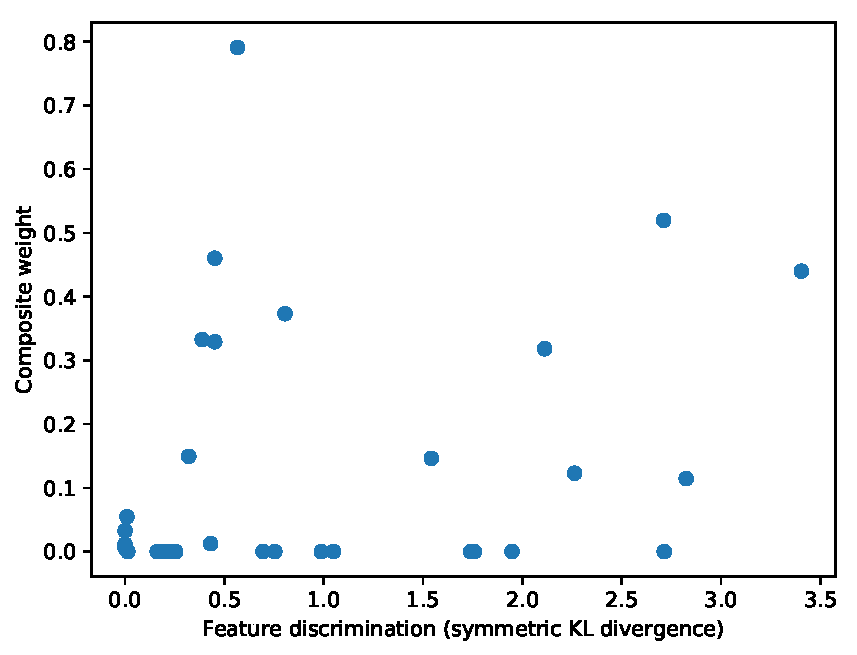
\includegraphics[width=.6\textwidth]{disc_weight_plot.pdf}
  \end{center}
\caption{Distribution of optimal composite weights vs individual feature discrimination power in a binary classification task (breast cancer UCI dataset). Discrimination is measured by the maximum KL divergence between class-conditional generative distributions.}
\label{fig:disc_weight_plot}
\end{figure}

As is customary and is generally good practice, the training examples may be weighted in~(\ref{eq:train_likelihood}) so that the empirical distribution of classes matches the prior~$\pi(x)$ (enforcing balanced classes if the prior is uniform). Also, some regularization may be useful for stability: we shall in practice maximize $U(\lambda)-\alpha \|\blambda\|^2$, where $\alpha>0$ is a small damping factor.

Other training variants that we mention here but do not particularly recommend for interpretability include adding basis functions to the exponential family. For instance, class-dependent offsets may be added so as to learn the ``prior'' together with the composite weights. It is also possible to perform unconstrained optimization to achieve higher training likelihood, meaning that some composite weights are then negative.


\subsection{Maximum entropy interpretation}

Exponential family properties also imply that maximum likelihood training~(\ref{eq:train_likelihood}) is dual to a maximum entropy problem or, more precisely, an $I$-projection \cite{Csiszar-84}:
\begin{equation}
\label{eq:maxent}
\min_{p\in{\cal P}} D(p\|\pi \cdot h) = \sum_{x\in{\cal X}}\sum_{y\in{\cal Y}} p(x,\y) \log \frac{p(x,\y)}{\pi(x)h(\y)},
\end{equation}
subject to the constraints $p(\y)=h(\y)$ and $\E_p[\bell] \succeq \E_h[\bell]$, where 
${\cal P}$ is the set of joint probability distributions on ${\cal X}\times {\cal Y}$
with ${\cal Y}=\{\y_1,\ldots,\y_N\}$ the set of training data values, $h(x,\y)$ is the joint empirical distribution of targets and data, and $h(\y)$ is the corresponding marginal data distribution. Note that the constraints implicitly approximate the data marginal and the mean log-likelihood values by empirical estimates, suggesting the need for regularization on small training sets.

The marginal constraint $p(\y)=h(\y)$ makes the $I$-projection equivalent to a maximum entropy classifier \cite{BergerA-96}, ensuring that only the conditional distribution $p(x|\y)$ is optimized. The mean log-likelihood constraints $\E_p[\bell] \succeq \E_h[\bell]$ encapsulate dependences between the target and the data, and consider a model admissible if it guarantees the same average log-likelihood levels as observed separately for each feature. This is weaker a constraint than assuming that the feature generative models $p(z_i|x)$ are true: it only assumes that the ``description length'' \cite{Grunwald-07} achieved by each agent is truthworthy.

%In the $I$-projection framework, the composite weights are the Lagrange multipliers associated with the mean log-likelihood inequality constraints.

A particularly insightful analysis given in \cite{Grunwald-04} shows that the $I$-projection is under broad conditions a minimax strategy for prediction according to the log loss. Hence, any $I$-projection is in some sense a best possible predictive model under particular constraints (in the limit of validity of empirical approximations). Our training of composite weights relates to multinomial logistic regression, another maximum entropy classifier, only differing by the choice of constraints, which, in the latter case, are not related to generative models.

As an alternative to the strategy considered here, the mean log-likelihood constraints may be expressed for each class rather than being averaged with respect to the prior, leading to a more general predictive model that we call ``super composite likelihood'', in which the weights become class-dependent (see Appendix~\ref{appendix:super}). This variant has the potential for higher prediction performance, but poses some conceptual difficulties, in particular that of having to define an arbitrary reference class. 

%used to predict whether breast lumps are benign or malignant based on a set of features extracted from fine-needle aspirate images.

%The most discriminative features tend to get large weight, however some quite discriminative features may get low weight if strongly correlated with a more discriminative feature

%Non-linear means that features with average discrimination power may get low weight as they are superseded by the most discriminative features. But some features with low discrimination power may also get large weight, which does not mean that they are very influential in practice (see above). This is illustrated in Figure~\ref{fig:disc_weight_plot} with the UCI breast cancer dataset. 

%{\color{red} Equality constraints (negative weights) are less interpretable.}

%{\color{red} Offsets.}

%{\color{red} Data weights.}

%Need to weight the data to adjust to prior as a general measure when minimizing cross-entropy, which should yield a conditional model that approximates the ``true'' conditional distribution, $q(x|y)\approx p(x|y)$. So the model will absorb the ``true'' marginal of $x$, which should thus be replaced by the prior if we want the model to mimic ideal Bayesian inference. In our case, it means that the composite likelihood approximates the true likelihood.

%We can further enforce exact prior matching by including offsets ($K-1$ free parameters), in which case the training phase learns $\pi(x)$ so that it matches the prior $\pi(x)$ in the sense $\int h(\y)p_\lambda(x|y)dy = \pi(x)$. This ``deforms'' the prior to improve the training score. But why is it important to enforce this constraint? Again, it all makes things just less interpretable. 

%When including offsets, using homoscedastic generative variance estimation and equality constraints, composite likelihood is equivalent to binomial logistic regression. However, equality constraints are not easily interpretable.

%In some sense, composite weights replace the multiple testing correction required in the frequentist inference paradigm for proper control of false positives. Here, we don't control false positives, we control prediction accuracy.

%Why not using the feature-based posteriors or Bayes factors rather than the likelihoods? It's a possibility (perhaps a connection here with Gr\"unwald's luckiness). A justification for not doing it is that the coordinator should discard the priors used by the agents. The constraints are not purely evidence-based since the moments depend on the coordinator's prior but it is arguable a mess of priors wouldn't be good.

%Single feature case ($y=z$): the maxent solution has the form $p(x|y)\propto\pi(x)p(\y|x)^\lambda$. We expect to have $\lambda=1$ but it's not necessarily the case. It is if $h(\y)=\int\pi(x)p(\y|x)dx$ because then $h(\y)p(x|y)=\pi(x)p(\y|x)$ so the constraint is verified (and active). This also tells us that the data marginal should be consistent with the prior on labels for this much expected consistency property to hold. So, either weight datapoints so as to match a desired prior (e.g., uniform) or take the empirical distribution of labels as the ``prior''. 

%Which brings another question: in this case, the (unique) weight is insensitive to the prior -- is it true in general? The answer is no. The weights generally depend on the prior. Hence the maxent composite likelihood is prior-dependent. This is an important conceptual difference with the classical notion of likelihood.



\section{Discussion}
\label{sec:discussion}

It is easy to build a good classifier. You just need to pick a parametric family that is big enough to produce a good fit yet small enough to avoid overfitting. Less easy is to interpret what the classifier does. Deep learning is cool but it is relevant to AI only if the representations it learns are generic enough to be used in other problems, i.e. it should ultimately be validated via transfer learning.

{\color{red} Why prediction performance is still important? Because it validates (or not) interpretation. Interpretation is the goal but prediction performance is a crucial intermediate step.}

{\color{red} We cannot rank features according to their weights. A feature might incidentally get a large weight because its likelihood is flat. Feature relevance also depends on conditional likelihood distribution. Consider mutually independent features: each one recieves a unit weight, but some may be independent from target.}

{\color{red} Can we use the same dataset to learn both the feature generative distributions and the composite weights? In principle, nothing speaks against this.} 

{\color{red} Semi-generative method. Good for shallow learning or transfer learning. Still need representation learning methods.}

{\color{red} Alternative to logistic regression in deep learning? Would require a game-theoretic learning approach... future work.} 

{\color{red} Composite Bayes is invariant by affine transformation of the data (unlike multinomial LR, which is problematic when damping is applied).}

{\color{red} Is damping important? (it guarantees training cost is stricly convex).}

{\color{red} Can we interpret maximum weight likelihood as a ``maximum relevance minimum redudancy'' feature selection approach?}

%In other words, is $\bar{a}(\blambda)$ a measure of feature redundancy? At fixed $\y$, if one $\lambda_i\to\infty$, then $a(\blambda,\y)\ot\infty$ except if $\ell_i(x,\y)\preceq 0$, in which case it goes to $-\infty$. If using likelihood ratios, this only happens if the reference class is the most likely for $\y$. But then we can prove that it can't happen for all $\y$ (otherwise the associated moment would be negative), so basically $\bar{a}(\blambda)$ blows up when at least one weight gets large. And if several weights get large simultaneously, then it blows up even more so we might consider it a redundancy measure to some extent...

Some experimental observations. In the iris dataset (historical data used by Fisher to demonstrate linear discriminant analysis), composite Bayes finds that petal length is the most relevant feature followed by petal width, while sepal length and width get zero weight. In the wine dataset, the flavanoids is the most relevant feature for standard composite Bayes, but it's color intensity closely followed by flavanoids for the super composite version. In the breast cancer, both approaches are equivalent since it is a binary problem, weights are very sparse: only 13/30 are non-zero with worst area the most relevant. In the digits prolem, the most relevant features tend to be in the image center; composite Bayes can achieve similar performance to multinomial logistic regression with about 10 times less parameters.

Number of independent discriminative parameters in logistic regression: $(K-1)(F+1)$. In standard composite inference: $F$ (or $K-1+F$ with offsets). Difference $=(K-2)(F+1)+1$ (or $=(K-2)F$). In super-composite inference: $(K-1)(F+1)$ (if reference is a class). Number of generative parameters in composite inference using univariate Gaussian models: $2K$ with heteroscedasticity, $K+1$ with homoscedasticity.

Intuition behind weights: notion of global feature relevance. But does $\lambda_1>\lambda_2$ imply that $z_1$ is more relevant than $z_2$ for a particular instance? No. But we can assess the influence of each scaled likelihood in order to rank features according to their influence on the decision.

CL is a concept from computational statistics that has mainly been developed so far in a frequentist perspective as a surrogate for the maximum likelihood method. We have shown a deep connection between CL and probabilistic inference, thereby establishing CL as a class of discriminative models. Because CL is built from a set of marginal feature-specific generative distributions, it is in essence a two-step semi-generative, semi-discriminative learning approach. In the first, ``generative'' phase, the feature distributions are learned; in the second, ``discriminative'' phase, the feature weights are learned. This strategy can be thought of as a form of non-adaptive boosting.

%The first phase corresponds to the training of ``weak learners''. The second phase amounts to a form of boosting. 

A purely discriminative learning could be used instead but...
Why potentially more efficient than pure discriminative training: because generative training is always more efficient than discriminative training if models are comparable. So the key point is that ``we have less parameters in the discriminant phase". Good in small datasets. But also in asymptotic regime if the features are weakly or highly correlated (???).

Logistic regression / naive Bayes example. Under homoscedasticity (assuming that each feature has class-independent variance), CBI is equivalent to logistic regression -- because the predictive distribution family is the same. This is a case where BCI brings nothing. But consider heteroscedasticity, then BCI yields a quadratic classifier. Compared to a fully discriminative model, the number of parameters to learned in the discriminative phase is reduced by half.

The first training phase is easier if supervised but could be unsupervised too (using mixture models). How do we then deal with label switching issues? Can we safely assume conditional feature independence {\em in the generative training phase}? I believe so provided that the marginal distribution parameters are disjoint. It's obvious in the supervised learning scenario.

If unsupervised, the first learning phase could be compared with contrastive pre-training of RBMs \cite{Hinton-06,Fischer-14}, which also optimize parameters for generation of observable features. BCI is comparable with an RBM with a single output unit (which is just a generative model assuming conditionial feature independence). The key difference is that the RBM is a full generative model while BCI only deals with marginal models, hence relying on weaker assumptions. This won't change anything in the pre-training phase but RBMs have to deal with more parameters in the generative learning phase. In fully supervised context, RBM pre-training is pointless since all parameters learned in the first phase will be overwritten. In BCI, pre-training is crucial even in supervised context because the parameters learned in the discriminative phase (the feature weighs) describe a sub-manifold of the predictive distribution family.

Needs features. Not a representation learning method, but could be coupled why not.


%{\color{red} Moreover, while RBM parameters are typically refined in a supervised discriminative learning step, disjoint set of parameters for SCL. Dunno how to say that.} 

%In such context, SCL competes with classical discriminative models (logistic regression, Gaussian processes \cite{Rasmussen-06}, maximum entropy models \cite{BergerA-96}, etc.), and may compare more or less favorably in practice depending on the amount of training data. For relatively small training datasets, we may hope for more accurate inference using~SCL than using traditional discriminative models, extrapolating from the results of \cite{Ng-01} regarding the comparison between logistic regression and na\"ive Bayes classifiers.
%{\color{red}Ici, il manque la comparaison avec les RBMs qui ne sont pas (forcement) des modeles discriminatifs.}

%%, hence alleviating the need for heavily supervised model training

%In summary, CL has the potential to yield weakly supervised or unsupervised Bayesian-like inference procedures depending on the particular task at hand. This property reflects the encoding of statistical relationships between the data and {\em all} unknown parameters. CL thus appears as a trade-off between generative models, which are optimal for unsupervised learning but possibly intractable, and traditional discriminative models (logistic regression, Gaussian processes \cite{Rasmussen-06}, maximum entropy models \cite{BergerA-96}, etc.), which are inherently supervised. CL models are discriminative models assembled from atomic generative models and, from this point of view, may be considered as {\em semi-generative} models.

%CL may be considered as a {\em semi-generative} model: a discriminative model assembled from partial generative models.

%As a note of caution, we shall stress that the pre-determined weights assigned to the different associations between observed and unobserved values represent prior knowledge regarding the informativeness of clues. A poor choice of weights will inevitably result in a poor approximation to the ``true'' Bayesian posterior -- the posterior that would be obtained from a realistic generative model if it was tractable. In future work, we will investigate feature selection strategies to mitigate this problem.

% Improve the discussion on following aspects:
% ** Why is it compatible with unsupervised learning? Give more insight.
% ** Stress the contribution: class-specific weighting.
% * Pivotality argument.
% * Bayes is a special case of composite Bayes.

{\color{red}Product of fucking experts \cite{Hinton-02}. Log-linear pool to build a generative model (assuming in fact independence between experts). Better seen as a ``log-mixture model''. Sounds like each expert is associated with a class, so it's the same as a RBM. Contrastive learning approximates ML parameter estimation. The experts are learning jointly. It's just a generative model.}

{\color{red}Two-step training: generative phase then discriminative phase. Why is it cool?}

{\color{red}CBI is just a way to reweight Naive Bayes. What's the big deal? Can we really expect massively superior performance? Are we just talking about realistic credibility sets?}

Future work: can we collapse generative and discriminative training into a single step? Maybe using the concept of {\em minimally informative likelihood} \cite{Yuan-99b}.


\appendix


\section{Basic frequentist properties of composite likelihood}
\label{appendix:frequentist}

Let a multivariate observable variable~$\y \sim p(\y|x_\star)$ distributed according to some target value~$x_\star$. For any extracted feature~$z_i$ and any hypothetical target value~$x$, the following double inequality holds:
$$
0 \leq
E\left[
\log \frac{p(z_i|x_\star)}{p(z_i|x)}
\right]
\leq
E\left[
\log \frac{p(\y|x_\star)}{p(\y|x)}
\right],
$$
where the expectation is taken with respect to the true distribution $p(\y|x_\star)$. This fact follows from two basic properties of KL~divergence: positivity and partition inequality.

Using a weighted sum of such inequalities, we can bracket the expected variations of the logarithm of any composite likelihood function~(\ref{eq:comp_lik}) with positive weights~$\blambda\succeq 0$:
\begin{equation}
\label{eq:variation_bound}
0 \leq
E\left[ \log \frac{L_c(x_\star, \blambda)}{L_c(x,\blambda)} \right]
\leq 
s_\blambda E\left[ \log \frac{L(x_\star)}{L(x)} \right]
,
\end{equation}
with $s_\blambda\equiv \|\blambda\|_1 =\sum_i \lambda_i$, and $L(x)$ the true likelihood function, {\em i.e.} $L(x)\equiv \log p(\y|x)$.

This implies two general asymptotic properties of composite likelihood:
\begin{itemize}
\item {\em Consistency.} The expected composite log-likelihood is maximized by~$x_\star$.
\item {\em Conservativeness for unit sum weights.} If the weights sum up to one or less ($s_\blambda\leq 1$), composite likelihood ratios of the true target~$x_\star$ vs.~other target values~$x$ tend to be underestimated, {\em i.e.} are smaller on the average than corresponding true likelihood ratios.
\end{itemize}


\section{Conditional composite likelihood}
\label{appendix:conditional}

As a straightforward  extension of marginal CL, each feature-based likelihood may be conditioned by an additional ``independent'' feature $z^c_i = f^c_i(\y)$ considered as a predictor of the ``dependent'' feature, $z_i=f_i(\y)$, yielding the more general form:
\begin{equation}
\label{eq:cond_feat_lik}
\ell_i(x) = p(z_i|x,z^c_i).
\end{equation}

Conditioning may be useful if it is believed that $z^c_i$ alone is little or not informative about $x$, but can provide relevant information when considered jointly with $x$, as in the case of regression covariates, for instance. Equation~(\ref{eq:comp_lik}) then amounts to conditional CL \cite{Varin-11}, a more general form of CL also including Besag's historical {\em pseudo-likelihood} \cite{Besag-74} developed for image segmentation.


\section{Composite likelihood training}
\label{appendix:training}

Using the same notation as in Section~\ref{sec:training}, the likelihood function in~(\ref{eq:train_likelihood}) can be expanded as follows:
$$
U(\blambda) 
= \sum_{k=1}^N \left[
\log \pi(x_k) + \blambda^\top \bell(x_k, \y_k) - a(\blambda,\y_k)
\right]
$$

Maximizing $U(\blambda)$ is therefore equivalent to maximizing: 
$$
\psi(\blambda) \equiv \blambda^\top \bar{\bell} - \bar{a}(\blambda), 
$$
with:
$$
\bar{\bell} \equiv \frac{1}{N} \sum_k \bell(x_k,\y_k),
\qquad
\bar{a}(\blambda) \equiv \frac{1}{N} \sum_k a(\blambda,\y_k).
$$

Note that $\psi(\blambda)$ is nothing but the dual function associated with the maxent problem~(\ref{eq:maxent}). 

Derivatives...
$$
\nabla\psi(\blambda)
= \bar{\bell} - \frac{1}{N} \sum_k \nabla a(\blambda,\y_k) 
$$

$$
\nabla\nabla^\top\psi(\blambda)
= - \frac{1}{N} \sum_k \nabla \nabla^\top a(\blambda,\y_k)  
$$

We have:
$$
\nabla a(\blambda,\y) = \E_{\blambda}(\bell|\y),
\qquad
\nabla \nabla^\top a(\blambda,\y) = \text{Var}_{\blambda}(\bell|\y)
$$
proving that $a(\blambda,\y)$ is convex in $\blambda$ for any $\y$, and in turn proves the concavity of $\psi$.

To see this, let:
$$
z(\blambda,\y) 
\equiv e^{a(\lambda,\y)}  
= \sum_{x\in{\cal X}} \pi(x) e^{\blambda^\top \bell(x,\y)}
$$

We have:
$$
\nabla a = \frac{\nabla z}{z}
$$

$$
\nabla\nabla^\top a 
= \left(
\frac{\nabla \nabla^\top z}{z} 
- \frac{\nabla z \nabla z^\top}{z^2}
\right)
$$

$$
\nabla z 
=
\sum_{x\in{\cal X}} \pi(x) \bell(x,\y)  e^{\blambda^\top \bell(x,\y)}
$$

$$
\nabla \nabla^\top z 
=
\sum_{x\in{\cal X}} \pi(x) \bell(x,\y) \bell(x,\y)^\top e^{\blambda^\top \bell(x,\y)}
$$


\section{Super composite likelihood}
\label{appendix:super}

When chosen for computational simplicity, features may not only convey limited information at individual level, their informativeness may also be very much class-dependent. Consider, for instance, diagnosing a disease from a routine medical checkup. Body temperature may point to a bacterial infection by comparison with normality, but would not help detecting a non-infectious cardiovasc ular disease -- and conversely for, say, blood pressure. 

This motivates a more general pooling than the common log-linear pool~(\ref{eq:log_pool}) where features can be weighted depending on the target variable:
$$
p_\lambda(x|\y) \propto \pi(x) \prod_i \left[\frac{p(z_i|x)}{p_0(z_i)}\right]^{\lambda_i(x)},
$$
where $p_0$ is an arbitrary reference feature distribution (which is implicit if weights are class-independent as it is then effectless). Make sense to have a reference as it gives a customizable baseline for detection. Can be the feature distribution averaged over all classes (not recommended I would say) or the distribution of a particular class if that makes sense (e.g. healthy population). In this case, the super composite likelihood is equivalent to the standard one in the two-class case.

We can train this model by maximum likelihood, yielding a similar optimization problem as in Section~\ref{sec:training}. 

%If some classes are merged or split, then the other classes keep the same weights (assuming $h(\y)$ is kept constant, so we need to make sure the prior is adapted accordingly)! So if a patient was found to have 10 times more probability to be MCI than healthy (and healthy is the reference class), and we later split AD population into, say, pure AD and mixed AD, the MCI probably ratio fact will remain.

Super composite likelihood is essentially about combining binary versions of composite likelihood. It is analogous to the ``one-versus-rest'' strategy in multiple logistic regression. 

Link with PDF projection \cite{Baggenstoss-03}.

Advantages: richer model (so better predictions), probabilty ratios stable to class addition. Drawbacks: require a reference, no more consistency. Still interpretable, that's why it is worthwile mentioning.



\section{Log-likelihood ratio}

$$
\log r = \log \frac{N(x;\mu_1,\sigma_1)}{N(x;\mu_0,\sigma_0)}
$$

$$
\log N(x;\mu,\sigma) = -\frac{1}{2}\left[
\log(2\pi\sigma^2) + \frac{(x-\mu)^2}{\sigma^2}
\right]
$$

$$
\log r = -\frac{1}{2}
\left[
\log \frac{\sigma_1^2}{\sigma_0^2}
+ \frac{(x-\mu_1)^2}{\sigma_1^2} - \frac{(x-\mu_0)^2}{\sigma_0^2}
\right]
$$

It follows:
\begin{eqnarray*}
\log r 
 & = & 
-\frac{1}{2}\left[
\log \frac{\sigma_1^2}{\sigma_0^2}
+ \frac{\sigma_0^2(x-\mu_1)^2 - \sigma_1^2(x-\mu_0)^2}{\sigma_0^2 \sigma_1^2}
\right] \\
 & = & 
\frac{1}{2}\left[
\log \rho^2
+ \frac{(\rho^2-1)x^2 - 2(\rho^2\mu_0-\mu_1)x+ (\rho^2\mu_0 ^2-\mu_1^2)}{\sigma_0^2}
\right]
\end{eqnarray*}
with $\rho=\sigma_1/\sigma_0$. In the case of same variance ($\rho=1$), this simplies to an affine function of $x$ with offset given by the center of $(\mu_0,\mu_1)$:
$$
\log r = \frac{\mu_1-\mu_0}{\sigma^2} \left(
x - \frac{\mu_0 + \mu_1}{2}
\right) 
$$

In any case,
$$
E[\log r | H_1] = 
\frac{1}{2}
\left[
- \log \frac{\sigma_1^2}{\sigma_0^2}
+ \frac{\sigma_1^2 + (\mu_1-\mu_0)^2}{\sigma_0^2}
- 1
\right]
$$

Let $\delta = (\mu_1-\mu_0)/\sigma_0$. We have:
$$
E[\log r | H_1] = 
\frac{1}{2}
\left[
\delta^2
- \log \rho^2
+ \rho^2  - 1
\right]
$$




\bibliographystyle{abbrv}
\bibliography{cvis,stat,alexis}

%%\documentclass[english]{scrartcl}

\usepackage{fullpage}
\usepackage{amstext,amssymb,amsmath,amsthm}
\usepackage{graphicx,subfigure}
\usepackage{multirow}
\usepackage{url}
\usepackage{hyperref}
\usepackage{color}

\graphicspath{{.}{pics/}}

%\newtheorem{theorem}{Theorem}[section]
%\newtheorem{proposition}[theorem]{Proposition}


\title{Composite Bayesian inference}
\date{}
\author{Alexis Roche\thanks{\url{alexis.roche@centraliens.net}}}

%\newcommand{\fix}{\marginpar{FIX}}
%\newcommand{\new}{\marginpar{NEW}}
%\newcommand{\matphi}{\boldsymbol{\Phi}} 
%\def\x{{\mathbf{x}}}
%\def\z{{\mathbf{z}}}
%\def\u{{\mathbf{u}}}
%\def\p{{\bar{\mathbf{p}}}}
%\def\q{{\bar{\mathbf{q}}}}



\begin{document}

\maketitle

\begin{abstract}
This note revisits the concept of composite likelihood from the perspective of probabilistic inference, and advocates a machine learning approach to tune the associated ``weights'', which stems naturally from a connection with the maximum entropy principle: the predictive distribution that maximizes conditional entropy relative to a given prior and subject to multiple mean log-likelihood inequality constraints is, up to a normalizing factor, the prior multiplied by a particular composite likelihood function, hence providing a ``composite'' extension of Bayes rule. We argue that composite Bayesian inference is a middle way between generative and discriminative approaches to statistical inference, which can be powerful in shallow learning and transfer learning problems.
\end{abstract}


\section{Introduction}
\label{sec:intro}

Classical frequentist and Bayesian inference paradigms rest upon the existence of a probabilistic data-generating model that is both empirically valid and computationally tractable. Because this is challenging for complex data, other inference models are commonly used in applied science: deliberately misspecified generative models, as in quasi-likelihood methods \cite{White-82,Walker-13} or na\"ive Bayes \cite{Ng-01}; data compression models as in minimum description length \cite{Grunwald-07}; and discriminative models\footnote{A {\em discriminative} model is a parametric family that describes the distribution of a variable of interest conditional on data, in contrast with a {\em generative} model, which describes the conditional distribution of data given the variable of interest.}, which currently dominate the field of artificial intelligence and typically require massive supervised learning -- these include classical techniques (maximum entropy classifiers \cite{BergerA-96}, support vector machines \cite{Vapnik-00}, Gaussian processes \cite{Rasmussen-06}) as well as most deep learning techniques \cite{Lecun-15,Goodfellow-16} with the exception of deep belief networks \cite{Hinton-06,Fischer-14}. 

A strong limitation of discriminative models is that they are not suitable for unsupervised learning or on-the-fly parameter estimation because they treat the data and the model parameters as {\em marginally independent}, meaning that the data conveys no information about the parameters unless the variable of interest is observed. This is illustrated in Figure~\ref{fig:graph_comparison} by the respective directed graph representations of generative and discriminative models. For the same reason, supervised learning in a discriminative model is less precise than in a generative model spanning the same family of posteriors, hence it is less effective in small training sets \cite{Ng-01}. Overall, pure discriminative models are of little use outside the context of big labeled data.

% p(x,y|theta) = p(x|y,theta)p(y|theta)

\begin{figure}[!ht]
\begin{center}
\subfigure[Generative model]{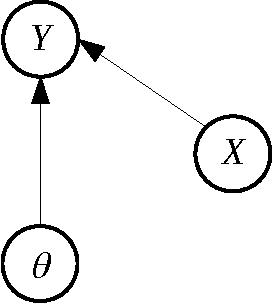
\includegraphics[width=.25\textwidth]{generative.pdf}\label{fig:generative}}
\hspace*{.2\textwidth}
\subfigure[Discriminative model]{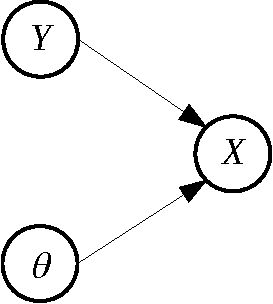
\includegraphics[width=.25\textwidth]{discriminative.pdf}\label{fig:discriminative}}
\caption{Bayesian networks representing generative and discriminative models, where $X$, $Y$ and $\theta$ respectively denote the variable of interest, the data, and the model parameters. Note the marginal independence of~$Y$ and~$\theta$ in the discriminative model.}
\label{fig:graph_comparison}
\end{center}
\end{figure}

Composite likelihood (CL, see \cite{Varin-11} and the references therein) is a semi-generative approach to statistical inference that extends the familiar notion of likelihood without requiring a full generative model. The key idea is to model an arbitrary set of low-dimensional features separately and then combine them, instead of modeling the data distribution as a whole. This may be viewed as a {\em divide and conquer} method to approximate the true but intractable likelihood. While maximum CL does not inherit the general property of maximum likelihood to yield an asymptotically minimum-variance estimator, it is consistent under mild conditions \cite{Xu-11} and may offer an excellent trade-off between computational and statistical efficiency in practice. 

In this note, CL is interpreted as a probabilistic opinion pool of ``agents'' making use of different pieces of information, or clues, extracted from the input data. Each agent acts as an isolated generative model-based statistician and expresses an opinion based on a single clue in the form of a likelihood function of the hidden variables. The agent opinions are then aggregated into a probability distribution on the hidden variables analogous to a Bayesian posterior.

We further argue that a particular log-linear opinion pool yields the best possible predictive distribution in the sense of maximum relative conditional entropy. This perspective entails a method to optimize the weights of the different agents from training data as in a typical discriminative learning scenario. 

%Something for true statisticians. Maybe we could clarify that we use the term ``Bayesian'' in the sense of ``empirical Bayesian'', implying that the parameters $\theta$ are to be estimated somehow contrary to a ``full Bayesian'' approach where they would be integrated out at inference time.


\section{Composite likelihood as opinion pooling}
\label{sec:pool}

Let $Y$ an observable multivariate random variable with sampling distribution $p(y|x)$ conditional on some unobserved variable of interest, $X\in{\cal X}$, where ${\cal X}$ is a known set. Given an experimental outcome $y$, the likelihood is the sampling distribution evaluated at $y$, seen as a function of $x$:
$$
L(x) = p(y|x)
.
$$

This requires a plausible generative model which, for complex data, may be out of reach or involve too many parameters to be estimated. A natural workaround known as {\em data reduction} is to extract some lower-dimensional representation $z=f(y)$, where $f$ is a many-to-one mapping, and consider the potentially more convenient likelihood function:
$$
\ell(x) = p(z|x)
.
$$

Substituting $L(x)$ with $\ell(x)$ boils down to restricting the sample space, thereby  ``delegating'' statistical inference to an ``agent'' provided with partial information. While it is valid for such an agent observing~$z$ only to consider $\ell(x)$ as the likelihood function of the problem, the drawback is that $\ell(x)$ might yield too vague a prediction of~$X$ due to the information loss incurred by data reduction. To make the trick statistically more efficient, we may extract several features, $z_i=f_i(y)$ for $i=1,2,\ldots,n$, and try to combine the likelihood functions $\ell_i(x) = p(z_i|x)$ that they elicit.

If we see the likelihoods as posterior distributions corresponding to uniform priors, this is a classical problem of probabilistic opinion aggregation from possibly redundant sources, for which several methods exist in the literature \cite{Tarantola-82,Genest-86,Garg-04,Allard-12}. We will show in Section~\ref{sec:maxent} that one that is particularly well-suited to our case is the {\em log-linear opinion pool}: 
\begin{equation}
\label{eq:log_pool}
p_\lambda(x|y) = \frac{1}{z_\lambda(y)} \pi(x) \prod_{i=1}^n p(z_i|x)^{\lambda_i},
\end{equation} 
where $\pi(x)$ is some reference distribution or prior, and $\lambda=(\lambda_1,\ldots,\lambda_n)$ is a vector of weights so that the normalizing factor:
$$
z_\lambda(y) = \int \pi(x) \prod_{i=1}^n p(z_i|x)^{\lambda_i} dx
$$
is finite, which holds whenever $\lambda\succeq 0$, {\em i.e.} all weights are positive, assuming that the agent opinions are always upper bounded. Negative weights should be ruled out as the existence condition $z_\lambda(y)<\infty$ would then depend on the particular opinions expressed by the agents. Also note that, while it is possible to have the weights depend on~$y$, there is a strong rational for constant weights as we shall see in the sequel. 

%Strictly positive weights guarantee the so-called 0/1 forcing property, that is, if an hypothesis~$x$ has zero likelihood according to at least one agent, then its consensus probability vanishes too.

% Not clear yet as to what a negative weight could mean!

The log-linear pool~(\ref{eq:log_pool}) bears a striking similarity to Bayes rule, yielding the form: $p_\lambda(x|y)\propto \pi(x) L^c_\lambda(x)$, where the quantity:
\begin{equation}
\label{eq:comp_lik}
L^c_\lambda(x) \equiv \prod_{i=1}^n \ell_i (x)^{\lambda_i}
\end{equation} 
plays the same role as a traditional likelihood function. This expression happens to be known in statistics as a {\em marginal composite likelihood} \cite{Varin-11}. See Appendix~\ref{sec:conditional} for the slightly more general form called {\em conditional composite likelihood}, which can be derived in the same way.

From~(\ref{eq:comp_lik}), we see that CL shares a convenient factorized form with the likelihood derived under the assumption of mutual feature independence, usually referred to as {\em na\"ive Bayes} or {\em simple Bayes} in the machine learning literature, which corresponds to the special case of unitary weights, $\lambda_1=\ldots=\lambda_n= 1$. The clear computational advantage of CL over the true likelihood is that it only requires to evaluate the marginal feature distributions rather than the joint distribution of all features.


\section{Tuning composite likelihood weights}

When the features can be considered exchangeable, it is natural to choose uniform CL weights. The CL is then a scaled version of the na\"ive Bayes likelihood, the common weight value being irrelevant to the maximum CL estimator (MCLE). The weight may be tuned so as to best adjust the pseudo posterior variance matrix to the asymptotic variance matrix of the MCLE \cite{Pauli-11}, or via a close-in-spirit curvature adjustment \cite{Ribatet-12}, in attempts to match the frequentist and composite Bayesian notions of uncertainty.

Ignoring such a goal, another frequent recommandation for CL weights is to sum up to one. This can be motivated in various ways. It turns out that the only pooling operator that does not explicitly depend on~$x$ and preserves {\em external Bayesianity} is the log-linear opinion pool with unit sum weights \cite{Genest-86b}. External Bayesianity essentially means that it should not matter whether the prior is incorporated before or after pooling, provided that all agents agree on the same prior. Another appealing property of log-linear pooling with unit sum weights is to minimize the average Kullback-Leibler (KL) divergence to the agent opinions \cite{Garg-04}. A maximum relative entropy property is also given in \cite{Wang-14}, Theorem~3.

Unit sum weights, however, correspond to the extreme situation where the features are assumed to be maximally redundant, but is clearly ineffective for independent or weakly correlated features, which require weights close to one for the CL to closely approximate the true likelihood. In this case, the CL may be much flatter than it should, leading to severly overestimated credibility sets.

{\color{red} Why is it important to fine-tune the weights?}
We therefore need a method to tune weights that can automatically adjust to the level of statistical dependence beween features.

%Instead, redundancy between agents is assumed by default, and is effectively encoded by the unit sum constraint on weights\footnote{Nevertheless, features which are {\em known} to be mutually independent can be merged into a single feature. This results in increasing their weights in the log-linear pool.}.

\section{Maxent composite likelihood}
\label{sec:maxent}

We can derive composite likelihood from the conditional maximum entropy principle \cite{BergerA-96}. It comes with a method of tuning weights, hence a particular composite likelihood function that we call maxent composite likelihood (MCL).

A cheap MaxEnt argument was already given by \cite{Wang-14}  (standard, non-conditional MaxEnt at fixed $y$, hence just an existence result but no feasible weight tuning).

What we do here is maximum {\em conditional} entropy. It's slightly more complex than a simple $I$-projection. The search space is a set of predictive distributions compatible with mean log-likelihood contraints. If I know the generative distribution, I know the expected log-likelihood.

We work with inequality constraints to force $\lambda\geq 0$:
$$
E[\log p(z_i|x)] \geq c_i \equiv \int \pi(x)p(z_i|x) \log p(z_i|x) dx dy
$$

What does the constraint mean? It means that a model is admissible if it compresses the data at least as well as all my agents. So we are not assuming that the generative models are {\em true}. We only assume that they are useful to compress the (reduced) data. Connection to MDL. 

Why not using the feature-based posteriors or Bayes factors rather than the likelihoods? It's a possibility (perhaps a connection here with Gr\"unwald's luckiness). A justification for not doing it is that the coordinator should discard the priors used by the agents. The constraints are not purely evidence-based since the moments depend on the coordinator's prior but it is arguable a mess of priors wouldn't be good.

Intuition behind weights: Lagrange multipliers to enforce a constraint... Notion of feature relevance. But does $\lambda_1>\lambda_2$ imply that $z_1$ is more relevant than $z_2$? 

The derivation assumed the marginal distribution of the data $h(y)$ to be known. In practice, it is estimated by the empirical distribution just like the moments are estimated.

Game theoretic interpretation \cite{Grunwald-04}.

The dual function boils down to the famous cross-entropy.

Single feature case ($y=z$): the maxent solution has the form $p(x|y)\propto\pi(x)p(y|x)^\lambda$. We expect to have $\lambda=1$ but it's not necessarily the case. It is if $h(y)=\int\pi(x)p(y|x)dx$ because then $h(y)p(x|y)=\pi(x)p(y|x)$ so the constraint is verified (and active). This also tells us that the data marginal should be consistent with the prior on labels for this much expected consistency property to hold. So, either weight datapoints so as to match a desired prior (e.g., uniform) or take the empirical distribution of labels as the ``prior''. 

Which brings another question: in this case, the (unique) weight is insensitive to the prior -- is it true in general? The answer is no. The weights generally depend on the prior. Hence the maxent composite likelihood is prior-dependent. This is an important conceptual difference with the classical notion of likelihood.

\section{Super composite likelihood}
\label{sec:super}

When chosen for computational simplicity, clues may not only convey limited information at individual level: their informativeness may also be very much hypothesis-dependent. Consider, for instance, diagnosing a disease from a routine medical checkup. Body temperature may point to a bacterial infection by comparison with normality, but would not help detecting a non-infectious cardiovascular disease -- and conversely for, say, blood pressure.

This motivates a more general setting where clues can be weighted differently depending on hypotheses.

What happens if we use mean-values constraints conditional on $x$ instead of jointly averaged over $x$ and $y$? This boils down to picking functions of the form:
$$
\chi(x-a)\ell_i(x,y)
$$

The answer is that the maxent solution has the form:
$$
p_\lambda(x|y) = \pi(x) \prod_i p(z_i|x)^{\lambda_i(x)}
$$

In other words, the weights become dependent on the variable of interest. This is the super composite likelihood idea.


\section{Composite EM algorithm for unsupervised learning}
\label{sec:gem}

In a nutshell: alternate unsupervised learning of partial model parameters ($M$-step) and re-estimation of label posteriors via maxent ($E$-step). 

$M$-step: given a posterior estimate $q(x|y)$, do just as if the features were independent and solve: 
$$
\max_\theta
\int \sum_i h(y)q(x|y) \log p_\theta(z_i,x) dx dy
$$

Note we can estimate cross-feature parameters such as class proportions.

Surrogate $E$-step: given generative parameters, recompute the moment constraints and update $q(x|y)$ according to the conditional maxent principle:
$$
\min_q
\int h(y)q(x|y) \log \frac{q(x|y)}{\pi(x)} dx dy
$$
s.t.
$$
\int h(y)q(x|y)\log p_\theta(z_i|x) dx dy \geq \int \pi(x)p_\theta(z_i|x)\log p_\theta(z_i|x) dx dy
$$

However, there is an important issue: how is $h(y)$ defined in both the $M$- and $E$-steps? In supervised context, $h(x,y)$ can be defined beforehand as the prior-corrected empirical distribution:
$$
h(x,y) = \pi(x) \frac{h_0(x,y)}{h_0(x)},
$$
where $h_0(x,y)$ is the raw empirical distribution. In unsupervised context, the best we can do is to replace $h_0(x,y)$ with $h_0(y)q(x|y)$, implying that the empirical distribution of $y$ is reweighted according to:
$$
h(y) = \sum_i w_i\delta(y-y_i),
\qquad
w_i = \int \pi(x)\frac{q(x|y_i)}{\sum_j q(x|y_j)} dx,
$$
which needs to be done each time $q(x|y)$ is updated, that is, after each $E$-step.

The other option is to keep $h(y)$ constant throughout the iterations but adapt $\pi(x)$ as the marginal distribution of labels learned in the $M$-step. In this case, it's no longer a ``prior''. 

Are we minimizing a unique functional as in the variational EM algorithm? Possibly not. We may see this generalization as a two-player game. One player tries to predict several data features independently. The other player tries to predict labels. Together, they find patterns (clusters) in unlabeled data. Does the more general version converge? Does the game have a value? And so on.

In the case of a single feature, is this the well-known EM? The $M$-step is clearly the same, what about the $E$-step? It is the same if $h(y)p_\theta(x|y)=p_\theta(y|x)\pi(x)$. However, this condition won't hold if $h(y)$ is an empirical distribution... In this special case, the ``E player'' could use the data distribution model produced by the ``M player'' instead of the empirical one but, more generally, there is no data distribution model so he has to stick to the empirical one.

The maxent is a surrogate for the $E$-step. It reflects the lack of a full model $p_\theta(x,y)$.

% Accounting here for Xi'An comment on xianblog.wordpress.com
% The sum of the powers is constrained to be equal to one, even though
% I do not understand why the dimensions of the projections play nog
% role in this constraint. Simplicity is advanced as an argument,
% which sounds rather weak…
%This simple constraint is implied by the external Bayesianity requirement: as it turns out, the only aggregation operator which is both externally Bayesian and independent from $x$ boils down to plugging a composite likelihood with unit sum weights into Bayes rule, hence extending the classical notion of likelihood in Bayesian analysis.


\section{Discussion}
\label{sec:discussion}

Deep learning is discriminative...

CL is a concept from computational statistics that has mainly been developed so far in a frequentist perspective as a surrogate for the maximum likelihood method. We have shown a deep connection between CL and probabilistic inference, thereby establishing CL as a class of discriminative models. Because CL is built from a set of marginal feature-specific generative distributions, it is in essence a two-step semi-generative, semi-discriminative learning approach. In the first, ``generative'' phase, the feature distributions are learned; in the second, ``discriminative'' phase, the feature weights are learned. This strategy can be thought of as a form of non-adaptive boosting.

%The first phase corresponds to the training of ``weak learners''. The second phase amounts to a form of boosting. 

A purely discriminative learning could be used instead but...
Why potentially more efficient than pure discriminative training: because generative training is always more efficient than discriminative training if models are comparable. So the key point is that ``we have less parameters in the discriminant phase". Good in small datasets. But also in asymptotic regime if the features are weakly or highly correlated (???).

Logistic regression / naive Bayes example. Under homoscedasticity (assuming that each feature has class-independent variance), CBI is equivalent to logistic regression -- because the predictive distribution family is the same. This is a case where BCI brings nothing. But consider heteroscedasticity, then BCI yields a quadratic classifier. Compared to a fully discriminative model, the number of parameters to learned in the discriminative phase is reduced by half.

The first training phase is easier if supervised but could be unsupervised too (using mixture models). How do we then deal with label switching issues? Can we safely assume conditional feature independence {\em in the generative training phase}? I believe so provided that the marginal distribution parameters are disjoint. It's obvious in the supervised learning scenario.

If unsupervised, the first learning phase could be compared with contrastive pre-training of RBMs \cite{Hinton-06,Fischer-14}, which also optimize parameters for generation of observable features. BCI is comparable with an RBM with a single output unit (which is just a generative model assuming conditionial feature independence). The key difference is that the RBM is a full generative model while BCI only deals with marginal models, hence relying on weaker assumptions. This won't change anything in the pre-training phase but RBMs have to deal with more parameters in the generative learning phase. In fully supervised context, RBM pre-training is pointless since all parameters learned in the first phase will be overwritten. In BCI, pre-training is crucial even in supervised context because the parameters learned in the discriminative phase (the feature weighs) describe a sub-manifold of the predictive distribution family.

Needs features. Not a representation learning method, but could be coupled why not.


%{\color{red} Moreover, while RBM parameters are typically refined in a supervised discriminative learning step, disjoint set of parameters for SCL. Dunno how to say that.} 

%In such context, SCL competes with classical discriminative models (logistic regression, Gaussian processes \cite{Rasmussen-06}, maximum entropy models \cite{BergerA-96}, etc.), and may compare more or less favorably in practice depending on the amount of training data. For relatively small training datasets, we may hope for more accurate inference using~SCL than using traditional discriminative models, extrapolating from the results of \cite{Ng-01} regarding the comparison between logistic regression and na\"ive Bayes classifiers.
%{\color{red}Ici, il manque la comparaison avec les RBMs qui ne sont pas (forcement) des modeles discriminatifs.}

%%, hence alleviating the need for heavily supervised model training

%In summary, CL has the potential to yield weakly supervised or unsupervised Bayesian-like inference procedures depending on the particular task at hand. This property reflects the encoding of statistical relationships between the data and {\em all} unknown parameters. CL thus appears as a trade-off between generative models, which are optimal for unsupervised learning but possibly intractable, and traditional discriminative models (logistic regression, Gaussian processes \cite{Rasmussen-06}, maximum entropy models \cite{BergerA-96}, etc.), which are inherently supervised. CL models are discriminative models assembled from atomic generative models and, from this point of view, may be considered as {\em semi-generative} models.

%CL may be considered as a {\em semi-generative} model: a discriminative model assembled from partial generative models.

%As a note of caution, we shall stress that the pre-determined weights assigned to the different associations between observed and unobserved values represent prior knowledge regarding the informativeness of clues. A poor choice of weights will inevitably result in a poor approximation to the ``true'' Bayesian posterior -- the posterior that would be obtained from a realistic generative model if it was tractable. In future work, we will investigate feature selection strategies to mitigate this problem.

% Improve the discussion on following aspects:
% ** Why is it compatible with unsupervised learning? Give more insight.
% ** Stress the contribution: class-specific weighting.
% * Pivotality argument.
% * Bayes is a special case of composite Bayes.

{\color{red}Product of fucking experts \cite{Hinton-02}. Log-linear pool to build a generative model (assuming in fact independence between experts). Better seen as a ``log-mixture model''. Sounds like each expert is associated with a class, so it's the same as a RBM. Contrastive learning approximates ML parameter estimation. The experts are learning jointly. It's just a generative model.}

{\color{red}Two-step training: generative phase then discriminative phase. Why is it cool?}

{\color{red}CBI is just a way to reweight Naive Bayes. What's the big deal? Can we really expect massively superior performance? Are we just talking about realistic credibility sets?}


\appendix

\section{Conditional composite likelihood}
\label{sec:conditional}

As a straightforward  extension of marginal CL, each feature-based likelihood may be conditioned by an additional ``independent'' feature $z^c_i = f^c_i(y)$ considered as a predictor of the ``dependent'' feature, $z_i=f_i(y)$, yielding the more general form:
\begin{equation}
\label{eq:cond_feat_lik}
\ell_i(x) = p(z_i|x,z^c_i).
\end{equation}

Conditioning may be useful if it is believed that $z^c_i$ alone is little or not informative about $x$, but can provide relevant information when considered jointly with $x$, as in the case of regression covariates, for instance. Equation~(\ref{eq:comp_lik}) then amounts to conditional CL \cite{Varin-11}, a more general form of CL also including Besag's historical {\em pseudo-likelihood} \cite{Besag-74} developed for image segmentation.


\section{Minimally discriminative model}

Let $\pi(x)$ some reference distribution that represents full
uncertainty about $X$. We wish to select the joint distribution
$p(x,y)$ that minimizes:
$$
I(p) = \int p(x,y) \log \frac{p(x|y)}{\pi(x)} dy,
$$ subject to feature mean-value constraints of the form:
$$
\int p(x,y) f(x,y) dx dy = \mu.
$$

There are two special cases of this problem in the literature.  On the
one hand, the {\em maximum entropy classifier} \cite{BergerA-96}
incorporates the constraint that $p(y)$ be known, however we will see
that this is not necessary. The {\em minimally informative likelihood}
method \cite{Yuan-99b,Yuan-99}, on the other hand, imposes that
$p(x)=\pi(x)$, hence assuming the form $p(x,y)=\pi(x)p(y|x)$. We won't
make such assumptions here and will consider the case where $\mu$ is
completely unknown.

The above problem is seen to be equivalent to minimizing the auxiliary
objective function:
$$
I(p,m) 
= \int p(x,y) \log \frac{p(x,y)}{\pi(x)m(y)} dxdy,
$$ over $p$ and $m$, subject to the same constraints on $p$. We note
that $I(p,m)=I(p)+D(p_y\|m)$, showing that the auxiliary function
essentially adds a penalty term to the actual objective in order to
force $p(y)$ close to $m(y)$.

Minimizing $I(p,m)$ along both $p$ and $m$ is basically a minimum KL
divergence problem between two convex distribution spaces, so there
must be a unique solution {\bf -- to be checked in
  \cite{Cover-91}}. It is similar to the rate-distortion problem in
information theory, which may be solved by alternate minimization,
yielding a Blahut-Arimoto algorithm.
\begin{itemize}
\item {\em Let's call it A-step}. Optimize $p(x,y)$ at fixed $m$
  s.t. constraint:
$$
\exists \lambda, \qquad
p_{\lambda,m}(x,y) = \frac{1}{Z(\lambda, m)} \pi(x) m(y) e^{-\lambda^\top t(x,y)}
$$
The actual $\lambda$ is found my maximizing the dual function
$\psi(\lambda,m)$, see below.
\item {\em Let's call it B-step}. Optimize $m(y)$ at fixed $p(x,y)$:
$$
m(y) = \int p(x,y) dx
$$
\end{itemize}

Upon convergence, the algorithm outputs both joint and marginal
distributions $p_{\star}(x,y)$ and $m_{\star}(y)$ that both depend on
$\mu$. By construction, we have that $p_{\star}(y) = m_{\star}(y)$,
therefore $p_\star(x|y)=p_{\star}(x,y)/m_{\star}(y)$.


\section{Comparison with maximum entropy classifier}

Lagrangian...
$$
{\cal L}(p,m,\lambda)
= 
\int p(x,y) \log \frac{p(x,y)}{\pi(x)m(y)} dxdy
+
\lambda^\top \left( 
\int p(x,y) f(x,y) dydy - \mu 
\right)
$$ where $\lambda$ represents a vector-valued Lagrange multiplier. At
fixed $m$, the solution has the form:
$$
p_{\lambda,m}(x,y) = \frac{1}{Z(\lambda,m)}
\pi(x) m(y) e^{-\lambda^\top f(x,y)} 
$$

Note that this implies that the conditional distribution is
independent of $m$ once $\lambda$ is determined,
$$
p_\lambda(x|y) = \frac{1}{z(\lambda,y)} \pi(x) e^{-\lambda^\top f(x,y)} 
$$

Also, the marginal is a modulation of $m(y)$:
$$
p_{\lambda,m}(y) = \frac{z(\lambda,y)}{Z(\lambda,m)} m(y)
$$

Dual function at fixed $m$:
$$
\psi(\lambda,m) 
\equiv \min_p {\cal L}(p,m,\lambda)
= 
- \log Z(\lambda,m) - \lambda^\top \mu
.
$$ 

An alternative expression is:
$$
\psi(\lambda, m)
= 
\int h(x,y) 
\log \frac{p_{\lambda,m}(x,y)}{\pi(x)m(y)} dxdy,
$$ where $h(x,y)$ is any distribution statisfying the
constraints. This shows that maximizing the dual function at fixed $m$
is essentially the same as minimizing the KL divergence
$D(h\|p_{\lambda,m})$ over $\lambda$, in other words fitting $h(x,y)$
by some distribution of the form $p_{\lambda,m}$. The fact that the
result does not depend on the particular $h(x,y)$ that is chosen, as
long as it satifies the constraint, is a general property of
exponential families.

We also have that the dual function associated with $I(p)$ reads:
\begin{eqnarray*}
\psi(\lambda) 
 & = & \min_m \psi(\lambda, m)\\
 & = & \int h(x,y) \log \frac{p_{\lambda}(x|y)}{\pi(x)} dxdy\\
 & = & -\int h(y) \log z(\lambda,y) dy - \lambda^\top \mu
\end{eqnarray*}

But, wait, that's exactly what we get in the maximum entropy
classifier! So, at the end of the day, we simply got an alternative
method to learn $\lambda$ in the maximum entropy classifier, i.e. the
Blahut-Arimoto algorithm as opposed to a brute-force maximization of
$\psi(\lambda)$. Both methods will converge to the same $\lambda$...

What it essentially means is that the optimal $\lambda$ is insensitive
to $m(y)$ as long as $m(y)$ is compliant in the sense that:
$$
m(y) = \int h(x,y) dx,
$$ for some distribution $h(x,y)$ statisfying the constraint. This is
true for the optimal $m_\star(y)$ output by the BA algorithm, but
also, for instance, for the empirical distribution of observations in
a training dataset used to estimate $\mu$, as proposed in
\cite{BergerA-96}. The only special property of $m_\star(y)$ is to
yield the full Bayesian model $p_\star(x,y)=p_\star(x|y)m_\star(y)$
that minimizes the discrimination information. We may not care too
much about that in practice since we will only use $p_\star(x|y)$. 

\section{Comparison with minimally informative likelihood}

Yuan \cite{Yuan-99} considered the situation where we add the
constraint that $p(x)=\pi(x)$ to the minimum discrimination inference
problem. Unknown is then the conditional distribution
$p(y|x)$. Lagrangian...
\begin{eqnarray*}
{\cal L}(p,m,\lambda)
 & = & 
\int \pi(x)p(y|x) \log \frac{p(y|x)}{m(y)} dxdy
+
\lambda^\top \left( 
\int \pi(x)p(y|x) f(x,y) dydy - \mu 
\right) \\
 & = & 
\int \pi(x)
\left( 
\int
p(y|x) \log \frac{p(y|x)}{m(y)} dy
+
\lambda^\top 
\int p(y|x) f(x,y) dy
- \mu 
\right)
dx 
\end{eqnarray*}

The derivative is given by,
$$
\frac{\partial\cal L}{\partial p(y|x)}
= 
\pi(x)\left[ 
1 + \log \frac{p(y|x)}{m(y)} 
+ \lambda^\top f(x,y)
\right],
$$
hence the optimal model at fixed $m$ has the form:
$$
p_{\lambda,m}(y|x) = \frac{1}{Z(\lambda,m,x)} m(y) e^{-\lambda^\top f(x,y)} 
$$

Note that the induced posterior distribution $p_{\lambda,m}(x|y)$ has
a different form from above unless the normalizing factor
$Z(\lambda,m,x)$ turns out independent from $x$. If this is not the
case, we no longer have the property that $p_{\lambda,m}(x|y)$ is
independent from $m$ given $\lambda$.

Dual function...
$$
\psi(\lambda,m) 
=
- \int \pi(x) \log Z(\lambda, m, x) dx
- \lambda^\top \mu
$$

Equivalently, for any distribution under the form $\pi(x)h(y|x)$ that
satisfies the moment constraint, we have:
$$
\psi(\lambda,m) 
=
\int \pi(x) h(y|x) \log \frac{p_{\lambda,m}(y|x)}{m(y)} dxdy
$$

Now, the real question is why should we constrain $p(x)$, which boils
down to a Bayesian prior in this context, to be the same as our
reference $\pi(x)$? It only makes sense if we want our inference to
stick to a generative modeling paradigm... but haven't we already
given up on that? Therefore, unless we find a good reason not to, we
won't impose the $p(x)=\pi(x)$ constraint, thereby allowing for a
discrepancy between the reference and the prior.


\section{Discriminative vs. semi-discriminative}

Let's go back to the equivalence we found between our approach and the
maximum entropy classifier (MCE) \cite{BergerA-96}. We have said that
the former is essentially a re-formulation of MCE.

But the re-formulation also conveys a generalization of MCE if,
instead of letting $m$ being an arbitrary distribution, we restrict
its search space to some set of acceptable reference
distributions. Would such a strategy be useful? 

Recall that the method selects the joint distribution that minimizes
discriminative information, as defined by $I(p)$:
$$
I(p) 
= \int p(x,y)\log\frac{p(x|y)}{\pi(x)} dxdy
= E_Y[D(p_{x|y}\|\pi)]
$$

The latter characterization reminds us that discriminative information
is defined in an average sense. The corresponding posterior $p(x|y)$
may not be conservative for some $y$, in particular those that are
unlikely under $p(y)$. It would be a problem if that's the case for
the particular data at hand. For that to happen rarely, the ideal
$p(y)$ would be the ``true'' marginal distribution of $Y$.

However, for vague mean value constraints, nothing may prevent the
optimal $m_\star(y)$ from departing significantly from that ideal
distribution. In fact, we can show that $m_\star(y)$ only has mass at
$y$ values that maximize $z(\lambda_\star,y)$, and is therefore likely
sparse. This is because $m_\star$ minimizes $\psi(\lambda_\star,m)$,
which is equivalent to maximizing $Z(\lambda_\star,m)$ and we have:
$$
Z(\lambda, m) = \int m(y) z(\lambda, y) dy.
$$

In other words, the solution to our problem may be singular! It does
not hurt since, as discussed above, one may alternatively fix $m(y)$
to some pre-defined distribution... but this, in practice, restricts
the method to supervised learning situations.

We may not face this issue with the MIL method, which further imposes
the prior on $X$, so all the information from the constraints goes
into specifying a possibly reasonable generative model.



\bibliographystyle{abbrv}
\bibliography{cvis,stat,alexis}

%%\documentclass[english]{scrartcl}

\usepackage{fullpage}
\usepackage{amstext,amssymb,amsmath,amsthm}
\usepackage{graphicx,subfigure}
\usepackage{multirow}
\usepackage{url}
\usepackage{hyperref}
\usepackage{color}

\graphicspath{{.}{pics/}}

%\newtheorem{theorem}{Theorem}[section]
%\newtheorem{proposition}[theorem]{Proposition}


\title{Composite Bayesian inference}
\date{}
\author{Alexis Roche\thanks{\url{alexis.roche@centraliens.net}}}

%\newcommand{\fix}{\marginpar{FIX}}
%\newcommand{\new}{\marginpar{NEW}}
%\newcommand{\matphi}{\boldsymbol{\Phi}} 
%\def\x{{\mathbf{x}}}
%\def\z{{\mathbf{z}}}
%\def\u{{\mathbf{u}}}
%\def\p{{\bar{\mathbf{p}}}}
%\def\q{{\bar{\mathbf{q}}}}



\begin{document}

\maketitle

\begin{abstract}
This note revisits the concept of composite likelihood from the perspective of probabilistic inference, and advocates a machine learning approach to tune the associated ``weights'', which stems naturally from a connection with the maximum entropy principle: the predictive distribution that maximizes conditional entropy relative to a given prior and subject to multiple mean log-likelihood inequality constraints is, up to a normalizing factor, the prior multiplied by a particular composite likelihood function, hence providing a ``composite'' extension of Bayes rule. We argue that composite Bayesian inference is a middle way between generative and discriminative approaches to statistical inference, which can be powerful in shallow learning and transfer learning problems.
\end{abstract}


\section{Introduction}
\label{sec:intro}

Classical frequentist and Bayesian inference paradigms rest upon the existence of a probabilistic data-generating model that is both empirically valid and computationally tractable. Because this is challenging for complex data, other inference models are commonly used in applied science: deliberately misspecified generative models, as in quasi-likelihood methods \cite{White-82,Walker-13} or na\"ive Bayes \cite{Ng-01}; data compression models as in minimum description length \cite{Grunwald-07}; and discriminative models\footnote{A {\em discriminative} model is a parametric family that describes the distribution of a variable of interest conditional on data, in contrast with a {\em generative} model, which describes the conditional distribution of data given the variable of interest.}, which currently dominate the field of artificial intelligence and typically require massive supervised learning -- these include classical techniques (maximum entropy classifiers \cite{BergerA-96}, support vector machines \cite{Vapnik-00}, Gaussian processes \cite{Rasmussen-06}) as well as most deep learning techniques \cite{Lecun-15,Goodfellow-16} with the exception of deep belief networks \cite{Hinton-06,Fischer-14}. 

A strong limitation of discriminative models is that they are not suitable for unsupervised learning or on-the-fly parameter estimation because they treat the data and the model parameters as {\em marginally independent}, meaning that the data conveys no information about the parameters unless the variable of interest is observed. This is illustrated in Figure~\ref{fig:graph_comparison} by the respective directed graph representations of generative and discriminative models. For the same reason, supervised learning in a discriminative model is less precise than in a generative model spanning the same family of posteriors, hence it is less effective in small training sets \cite{Ng-01}. Overall, pure discriminative models are of little use outside the context of big labeled data.

% p(x,y|theta) = p(x|y,theta)p(y|theta)

\begin{figure}[!ht]
\begin{center}
\subfigure[Generative model]{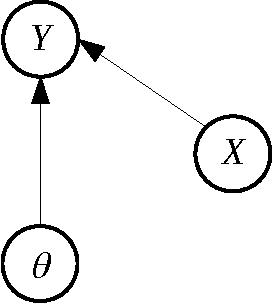
\includegraphics[width=.25\textwidth]{generative.pdf}\label{fig:generative}}
\hspace*{.2\textwidth}
\subfigure[Discriminative model]{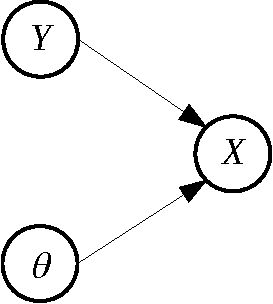
\includegraphics[width=.25\textwidth]{discriminative.pdf}\label{fig:discriminative}}
\caption{Bayesian networks representing generative and discriminative models, where $X$, $Y$ and $\theta$ respectively denote the variable of interest, the data, and the model parameters. Note the marginal independence of~$Y$ and~$\theta$ in the discriminative model.}
\label{fig:graph_comparison}
\end{center}
\end{figure}

Composite likelihood (CL, see \cite{Varin-11} and the references therein) is a semi-generative approach to statistical inference that extends the familiar notion of likelihood without requiring a full generative model. The key idea is to model an arbitrary set of low-dimensional features separately and then combine them, instead of modeling the data distribution as a whole. This may be viewed as a {\em divide and conquer} method to approximate the true but intractable likelihood. While maximum CL does not inherit the general property of maximum likelihood to yield an asymptotically minimum-variance estimator, it is consistent under mild conditions \cite{Xu-11} and may offer an excellent trade-off between computational and statistical efficiency in practice. 

In this note, CL is interpreted as a probabilistic opinion pool of ``agents'' making use of different pieces of information, or clues, extracted from the input data. Each agent acts as an isolated generative model-based statistician and expresses an opinion based on a single clue in the form of a likelihood function of the hidden variables. The agent opinions are then aggregated into a probability distribution on the hidden variables analogous to a Bayesian posterior.

We further argue that a particular log-linear opinion pool yields the best possible predictive distribution in the sense of maximum relative conditional entropy. This perspective entails a method to optimize the weights of the different agents from training data as in a typical discriminative learning scenario. 

%Something for true statisticians. Maybe we could clarify that we use the term ``Bayesian'' in the sense of ``empirical Bayesian'', implying that the parameters $\theta$ are to be estimated somehow contrary to a ``full Bayesian'' approach where they would be integrated out at inference time.


\section{Composite likelihood as opinion pooling}
\label{sec:pool}

Let $Y$ an observable multivariate random variable with sampling distribution $p(y|x)$ conditional on some unobserved variable of interest, $X\in{\cal X}$, where ${\cal X}$ is a known set. Given an experimental outcome $y$, the likelihood is the sampling distribution evaluated at $y$, seen as a function of $x$:
$$
L(x) = p(y|x)
.
$$

This requires a plausible generative model which, for complex data, may be out of reach or involve too many parameters to be estimated. A natural workaround known as {\em data reduction} is to extract some lower-dimensional representation $z=f(y)$, where $f$ is a many-to-one mapping, and consider the potentially more convenient likelihood function:
$$
\ell(x) = p(z|x)
.
$$

Substituting $L(x)$ with $\ell(x)$ boils down to restricting the sample space, thereby  ``delegating'' statistical inference to an ``agent'' provided with partial information. While it is valid for such an agent observing~$z$ only to consider $\ell(x)$ as the likelihood function of the problem, the drawback is that $\ell(x)$ might yield too vague a prediction of~$X$ due to the information loss incurred by data reduction. To make the trick statistically more efficient, we may extract several features, $z_i=f_i(y)$ for $i=1,2,\ldots,n$, and try to combine the likelihood functions $\ell_i(x) = p(z_i|x)$ that they elicit.

If we see the likelihoods as posterior distributions corresponding to uniform priors, this is a classical problem of probabilistic opinion aggregation from possibly redundant sources, for which several methods exist in the literature \cite{Tarantola-82,Genest-86,Garg-04,Allard-12}. We will show in Section~\ref{sec:maxent} that one that is particularly well-suited to our case is the {\em log-linear opinion pool}: 
\begin{equation}
\label{eq:log_pool}
p_\lambda(x|y) = \frac{1}{z_\lambda(y)} \pi(x) \prod_{i=1}^n p(z_i|x)^{\lambda_i},
\end{equation} 
where $\pi(x)$ is some reference distribution or prior, and $\lambda=(\lambda_1,\ldots,\lambda_n)$ is a vector of weights so that the normalizing factor:
$$
z_\lambda(y) = \int \pi(x) \prod_{i=1}^n p(z_i|x)^{\lambda_i} dx
$$
is finite, which holds whenever $\lambda\succeq 0$, {\em i.e.} all weights are positive, assuming that the agent opinions are always upper bounded. Negative weights should be ruled out as the existence condition $z_\lambda(y)<\infty$ would then depend on the particular opinions expressed by the agents. Also note that, while it is possible to have the weights depend on~$y$, there is a strong rational for constant weights as we shall see in the sequel. 

%Strictly positive weights guarantee the so-called 0/1 forcing property, that is, if an hypothesis~$x$ has zero likelihood according to at least one agent, then its consensus probability vanishes too.

% Not clear yet as to what a negative weight could mean!

The log-linear pool~(\ref{eq:log_pool}) bears a striking similarity to Bayes rule, yielding the form: $p_\lambda(x|y)\propto \pi(x) L^c_\lambda(x)$, where the quantity:
\begin{equation}
\label{eq:comp_lik}
L^c_\lambda(x) \equiv \prod_{i=1}^n \ell_i (x)^{\lambda_i}
\end{equation} 
plays the same role as a traditional likelihood function. This expression happens to be known in statistics as a {\em marginal composite likelihood} \cite{Varin-11}. See Appendix~\ref{sec:conditional} for the slightly more general form called {\em conditional composite likelihood}, which can be derived in the same way.

From~(\ref{eq:comp_lik}), we see that CL shares a convenient factorized form with the likelihood derived under the assumption of mutual feature independence, usually referred to as {\em na\"ive Bayes} or {\em simple Bayes} in the machine learning literature, which corresponds to the special case of unitary weights, $\lambda_1=\ldots=\lambda_n= 1$. The clear computational advantage of CL over the true likelihood is that it only requires to evaluate the marginal feature distributions rather than the joint distribution of all features.


\section{Tuning composite likelihood weights}

When the features can be considered exchangeable, it is natural to choose uniform CL weights. The CL is then a scaled version of the na\"ive Bayes likelihood, the common weight value being irrelevant to the maximum CL estimator (MCLE). The weight may be tuned so as to best adjust the pseudo posterior variance matrix to the asymptotic variance matrix of the MCLE \cite{Pauli-11}, or via a close-in-spirit curvature adjustment \cite{Ribatet-12}, in attempts to match the frequentist and composite Bayesian notions of uncertainty.

Ignoring such a goal, another frequent recommandation for CL weights is to sum up to one. This can be motivated in various ways. It turns out that the only pooling operator that does not explicitly depend on~$x$ and preserves {\em external Bayesianity} is the log-linear opinion pool with unit sum weights \cite{Genest-86b}. External Bayesianity essentially means that it should not matter whether the prior is incorporated before or after pooling, provided that all agents agree on the same prior. Another appealing property of log-linear pooling with unit sum weights is to minimize the average Kullback-Leibler (KL) divergence to the agent opinions \cite{Garg-04}. A maximum relative entropy property is also given in \cite{Wang-14}, Theorem~3.

Unit sum weights, however, correspond to the extreme situation where the features are assumed to be maximally redundant, but is clearly ineffective for independent or weakly correlated features, which require weights close to one for the CL to closely approximate the true likelihood. In this case, the CL may be much flatter than it should, leading to severly overestimated credibility sets.

{\color{red} Why is it important to fine-tune the weights?}
We therefore need a method to tune weights that can automatically adjust to the level of statistical dependence beween features.

%Instead, redundancy between agents is assumed by default, and is effectively encoded by the unit sum constraint on weights\footnote{Nevertheless, features which are {\em known} to be mutually independent can be merged into a single feature. This results in increasing their weights in the log-linear pool.}.

\section{Maxent composite likelihood}
\label{sec:maxent}

We can derive composite likelihood from the conditional maximum entropy principle \cite{BergerA-96}. It comes with a method of tuning weights, hence a particular composite likelihood function that we call maxent composite likelihood (MCL).

A cheap MaxEnt argument was already given by \cite{Wang-14}  (standard, non-conditional MaxEnt at fixed $y$, hence just an existence result but no feasible weight tuning).

What we do here is maximum {\em conditional} entropy. It's slightly more complex than a simple $I$-projection. The search space is a set of predictive distributions compatible with mean log-likelihood contraints. If I know the generative distribution, I know the expected log-likelihood.

We work with inequality constraints to force $\lambda\geq 0$:
$$
E[\log p(z_i|x)] \geq c_i \equiv \int \pi(x)p(z_i|x) \log p(z_i|x) dx dy
$$

What does the constraint mean? It means that a model is admissible if it compresses the data at least as well as all my agents. So we are not assuming that the generative models are {\em true}. We only assume that they are useful to compress the (reduced) data. Connection to MDL. 

Why not using the feature-based posteriors or Bayes factors rather than the likelihoods? It's a possibility (perhaps a connection here with Gr\"unwald's luckiness). A justification for not doing it is that the coordinator should discard the priors used by the agents. The constraints are not purely evidence-based since the moments depend on the coordinator's prior but it is arguable a mess of priors wouldn't be good.

Intuition behind weights: Lagrange multipliers to enforce a constraint... Notion of feature relevance. But does $\lambda_1>\lambda_2$ imply that $z_1$ is more relevant than $z_2$? 

The derivation assumed the marginal distribution of the data $h(y)$ to be known. In practice, it is estimated by the empirical distribution just like the moments are estimated.

Game theoretic interpretation \cite{Grunwald-04}.

The dual function boils down to the famous cross-entropy.

Single feature case ($y=z$): the maxent solution has the form $p(x|y)\propto\pi(x)p(y|x)^\lambda$. We expect to have $\lambda=1$ but it's not necessarily the case. It is if $h(y)=\int\pi(x)p(y|x)dx$ because then $h(y)p(x|y)=\pi(x)p(y|x)$ so the constraint is verified (and active). This also tells us that the data marginal should be consistent with the prior on labels for this much expected consistency property to hold. So, either weight datapoints so as to match a desired prior (e.g., uniform) or take the empirical distribution of labels as the ``prior''. 

Which brings another question: in this case, the (unique) weight is insensitive to the prior -- is it true in general? The answer is no. The weights generally depend on the prior. Hence the maxent composite likelihood is prior-dependent. This is an important conceptual difference with the classical notion of likelihood.

\section{Super composite likelihood}
\label{sec:super}

When chosen for computational simplicity, clues may not only convey limited information at individual level: their informativeness may also be very much hypothesis-dependent. Consider, for instance, diagnosing a disease from a routine medical checkup. Body temperature may point to a bacterial infection by comparison with normality, but would not help detecting a non-infectious cardiovascular disease -- and conversely for, say, blood pressure.

This motivates a more general setting where clues can be weighted differently depending on hypotheses.

What happens if we use mean-values constraints conditional on $x$ instead of jointly averaged over $x$ and $y$? This boils down to picking functions of the form:
$$
\chi(x-a)\ell_i(x,y)
$$

The answer is that the maxent solution has the form:
$$
p_\lambda(x|y) = \pi(x) \prod_i p(z_i|x)^{\lambda_i(x)}
$$

In other words, the weights become dependent on the variable of interest. This is the super composite likelihood idea.


\section{Composite EM algorithm for unsupervised learning}
\label{sec:gem}

In a nutshell: alternate unsupervised learning of partial model parameters ($M$-step) and re-estimation of label posteriors via maxent ($E$-step). 

$M$-step: given a posterior estimate $q(x|y)$, do just as if the features were independent and solve: 
$$
\max_\theta
\int \sum_i h(y)q(x|y) \log p_\theta(z_i,x) dx dy
$$

Note we can estimate cross-feature parameters such as class proportions.

Surrogate $E$-step: given generative parameters, recompute the moment constraints and update $q(x|y)$ according to the conditional maxent principle:
$$
\min_q
\int h(y)q(x|y) \log \frac{q(x|y)}{\pi(x)} dx dy
$$
s.t.
$$
\int h(y)q(x|y)\log p_\theta(z_i|x) dx dy \geq \int \pi(x)p_\theta(z_i|x)\log p_\theta(z_i|x) dx dy
$$

However, there is an important issue: how is $h(y)$ defined in both the $M$- and $E$-steps? In supervised context, $h(x,y)$ can be defined beforehand as the prior-corrected empirical distribution:
$$
h(x,y) = \pi(x) \frac{h_0(x,y)}{h_0(x)},
$$
where $h_0(x,y)$ is the raw empirical distribution. In unsupervised context, the best we can do is to replace $h_0(x,y)$ with $h_0(y)q(x|y)$, implying that the empirical distribution of $y$ is reweighted according to:
$$
h(y) = \sum_i w_i\delta(y-y_i),
\qquad
w_i = \int \pi(x)\frac{q(x|y_i)}{\sum_j q(x|y_j)} dx,
$$
which needs to be done each time $q(x|y)$ is updated, that is, after each $E$-step.

The other option is to keep $h(y)$ constant throughout the iterations but adapt $\pi(x)$ as the marginal distribution of labels learned in the $M$-step. In this case, it's no longer a ``prior''. 

Are we minimizing a unique functional as in the variational EM algorithm? Possibly not. We may see this generalization as a two-player game. One player tries to predict several data features independently. The other player tries to predict labels. Together, they find patterns (clusters) in unlabeled data. Does the more general version converge? Does the game have a value? And so on.

In the case of a single feature, is this the well-known EM? The $M$-step is clearly the same, what about the $E$-step? It is the same if $h(y)p_\theta(x|y)=p_\theta(y|x)\pi(x)$. However, this condition won't hold if $h(y)$ is an empirical distribution... In this special case, the ``E player'' could use the data distribution model produced by the ``M player'' instead of the empirical one but, more generally, there is no data distribution model so he has to stick to the empirical one.

The maxent is a surrogate for the $E$-step. It reflects the lack of a full model $p_\theta(x,y)$.

% Accounting here for Xi'An comment on xianblog.wordpress.com
% The sum of the powers is constrained to be equal to one, even though
% I do not understand why the dimensions of the projections play nog
% role in this constraint. Simplicity is advanced as an argument,
% which sounds rather weak…
%This simple constraint is implied by the external Bayesianity requirement: as it turns out, the only aggregation operator which is both externally Bayesian and independent from $x$ boils down to plugging a composite likelihood with unit sum weights into Bayes rule, hence extending the classical notion of likelihood in Bayesian analysis.


\section{Discussion}
\label{sec:discussion}

Deep learning is discriminative...

CL is a concept from computational statistics that has mainly been developed so far in a frequentist perspective as a surrogate for the maximum likelihood method. We have shown a deep connection between CL and probabilistic inference, thereby establishing CL as a class of discriminative models. Because CL is built from a set of marginal feature-specific generative distributions, it is in essence a two-step semi-generative, semi-discriminative learning approach. In the first, ``generative'' phase, the feature distributions are learned; in the second, ``discriminative'' phase, the feature weights are learned. This strategy can be thought of as a form of non-adaptive boosting.

%The first phase corresponds to the training of ``weak learners''. The second phase amounts to a form of boosting. 

A purely discriminative learning could be used instead but...
Why potentially more efficient than pure discriminative training: because generative training is always more efficient than discriminative training if models are comparable. So the key point is that ``we have less parameters in the discriminant phase". Good in small datasets. But also in asymptotic regime if the features are weakly or highly correlated (???).

Logistic regression / naive Bayes example. Under homoscedasticity (assuming that each feature has class-independent variance), CBI is equivalent to logistic regression -- because the predictive distribution family is the same. This is a case where BCI brings nothing. But consider heteroscedasticity, then BCI yields a quadratic classifier. Compared to a fully discriminative model, the number of parameters to learned in the discriminative phase is reduced by half.

The first training phase is easier if supervised but could be unsupervised too (using mixture models). How do we then deal with label switching issues? Can we safely assume conditional feature independence {\em in the generative training phase}? I believe so provided that the marginal distribution parameters are disjoint. It's obvious in the supervised learning scenario.

If unsupervised, the first learning phase could be compared with contrastive pre-training of RBMs \cite{Hinton-06,Fischer-14}, which also optimize parameters for generation of observable features. BCI is comparable with an RBM with a single output unit (which is just a generative model assuming conditionial feature independence). The key difference is that the RBM is a full generative model while BCI only deals with marginal models, hence relying on weaker assumptions. This won't change anything in the pre-training phase but RBMs have to deal with more parameters in the generative learning phase. In fully supervised context, RBM pre-training is pointless since all parameters learned in the first phase will be overwritten. In BCI, pre-training is crucial even in supervised context because the parameters learned in the discriminative phase (the feature weighs) describe a sub-manifold of the predictive distribution family.

Needs features. Not a representation learning method, but could be coupled why not.


%{\color{red} Moreover, while RBM parameters are typically refined in a supervised discriminative learning step, disjoint set of parameters for SCL. Dunno how to say that.} 

%In such context, SCL competes with classical discriminative models (logistic regression, Gaussian processes \cite{Rasmussen-06}, maximum entropy models \cite{BergerA-96}, etc.), and may compare more or less favorably in practice depending on the amount of training data. For relatively small training datasets, we may hope for more accurate inference using~SCL than using traditional discriminative models, extrapolating from the results of \cite{Ng-01} regarding the comparison between logistic regression and na\"ive Bayes classifiers.
%{\color{red}Ici, il manque la comparaison avec les RBMs qui ne sont pas (forcement) des modeles discriminatifs.}

%%, hence alleviating the need for heavily supervised model training

%In summary, CL has the potential to yield weakly supervised or unsupervised Bayesian-like inference procedures depending on the particular task at hand. This property reflects the encoding of statistical relationships between the data and {\em all} unknown parameters. CL thus appears as a trade-off between generative models, which are optimal for unsupervised learning but possibly intractable, and traditional discriminative models (logistic regression, Gaussian processes \cite{Rasmussen-06}, maximum entropy models \cite{BergerA-96}, etc.), which are inherently supervised. CL models are discriminative models assembled from atomic generative models and, from this point of view, may be considered as {\em semi-generative} models.

%CL may be considered as a {\em semi-generative} model: a discriminative model assembled from partial generative models.

%As a note of caution, we shall stress that the pre-determined weights assigned to the different associations between observed and unobserved values represent prior knowledge regarding the informativeness of clues. A poor choice of weights will inevitably result in a poor approximation to the ``true'' Bayesian posterior -- the posterior that would be obtained from a realistic generative model if it was tractable. In future work, we will investigate feature selection strategies to mitigate this problem.

% Improve the discussion on following aspects:
% ** Why is it compatible with unsupervised learning? Give more insight.
% ** Stress the contribution: class-specific weighting.
% * Pivotality argument.
% * Bayes is a special case of composite Bayes.

{\color{red}Product of fucking experts \cite{Hinton-02}. Log-linear pool to build a generative model (assuming in fact independence between experts). Better seen as a ``log-mixture model''. Sounds like each expert is associated with a class, so it's the same as a RBM. Contrastive learning approximates ML parameter estimation. The experts are learning jointly. It's just a generative model.}

{\color{red}Two-step training: generative phase then discriminative phase. Why is it cool?}

{\color{red}CBI is just a way to reweight Naive Bayes. What's the big deal? Can we really expect massively superior performance? Are we just talking about realistic credibility sets?}


\appendix

\section{Conditional composite likelihood}
\label{sec:conditional}

As a straightforward  extension of marginal CL, each feature-based likelihood may be conditioned by an additional ``independent'' feature $z^c_i = f^c_i(y)$ considered as a predictor of the ``dependent'' feature, $z_i=f_i(y)$, yielding the more general form:
\begin{equation}
\label{eq:cond_feat_lik}
\ell_i(x) = p(z_i|x,z^c_i).
\end{equation}

Conditioning may be useful if it is believed that $z^c_i$ alone is little or not informative about $x$, but can provide relevant information when considered jointly with $x$, as in the case of regression covariates, for instance. Equation~(\ref{eq:comp_lik}) then amounts to conditional CL \cite{Varin-11}, a more general form of CL also including Besag's historical {\em pseudo-likelihood} \cite{Besag-74} developed for image segmentation.


\section{Minimally discriminative model}

Let $\pi(x)$ some reference distribution that represents full
uncertainty about $X$. We wish to select the joint distribution
$p(x,y)$ that minimizes:
$$
I(p) = \int p(x,y) \log \frac{p(x|y)}{\pi(x)} dy,
$$ subject to feature mean-value constraints of the form:
$$
\int p(x,y) f(x,y) dx dy = \mu.
$$

There are two special cases of this problem in the literature.  On the
one hand, the {\em maximum entropy classifier} \cite{BergerA-96}
incorporates the constraint that $p(y)$ be known, however we will see
that this is not necessary. The {\em minimally informative likelihood}
method \cite{Yuan-99b,Yuan-99}, on the other hand, imposes that
$p(x)=\pi(x)$, hence assuming the form $p(x,y)=\pi(x)p(y|x)$. We won't
make such assumptions here and will consider the case where $\mu$ is
completely unknown.

The above problem is seen to be equivalent to minimizing the auxiliary
objective function:
$$
I(p,m) 
= \int p(x,y) \log \frac{p(x,y)}{\pi(x)m(y)} dxdy,
$$ over $p$ and $m$, subject to the same constraints on $p$. We note
that $I(p,m)=I(p)+D(p_y\|m)$, showing that the auxiliary function
essentially adds a penalty term to the actual objective in order to
force $p(y)$ close to $m(y)$.

Minimizing $I(p,m)$ along both $p$ and $m$ is basically a minimum KL
divergence problem between two convex distribution spaces, so there
must be a unique solution {\bf -- to be checked in
  \cite{Cover-91}}. It is similar to the rate-distortion problem in
information theory, which may be solved by alternate minimization,
yielding a Blahut-Arimoto algorithm.
\begin{itemize}
\item {\em Let's call it A-step}. Optimize $p(x,y)$ at fixed $m$
  s.t. constraint:
$$
\exists \lambda, \qquad
p_{\lambda,m}(x,y) = \frac{1}{Z(\lambda, m)} \pi(x) m(y) e^{-\lambda^\top t(x,y)}
$$
The actual $\lambda$ is found my maximizing the dual function
$\psi(\lambda,m)$, see below.
\item {\em Let's call it B-step}. Optimize $m(y)$ at fixed $p(x,y)$:
$$
m(y) = \int p(x,y) dx
$$
\end{itemize}

Upon convergence, the algorithm outputs both joint and marginal
distributions $p_{\star}(x,y)$ and $m_{\star}(y)$ that both depend on
$\mu$. By construction, we have that $p_{\star}(y) = m_{\star}(y)$,
therefore $p_\star(x|y)=p_{\star}(x,y)/m_{\star}(y)$.


\section{Comparison with maximum entropy classifier}

Lagrangian...
$$
{\cal L}(p,m,\lambda)
= 
\int p(x,y) \log \frac{p(x,y)}{\pi(x)m(y)} dxdy
+
\lambda^\top \left( 
\int p(x,y) f(x,y) dydy - \mu 
\right)
$$ where $\lambda$ represents a vector-valued Lagrange multiplier. At
fixed $m$, the solution has the form:
$$
p_{\lambda,m}(x,y) = \frac{1}{Z(\lambda,m)}
\pi(x) m(y) e^{-\lambda^\top f(x,y)} 
$$

Note that this implies that the conditional distribution is
independent of $m$ once $\lambda$ is determined,
$$
p_\lambda(x|y) = \frac{1}{z(\lambda,y)} \pi(x) e^{-\lambda^\top f(x,y)} 
$$

Also, the marginal is a modulation of $m(y)$:
$$
p_{\lambda,m}(y) = \frac{z(\lambda,y)}{Z(\lambda,m)} m(y)
$$

Dual function at fixed $m$:
$$
\psi(\lambda,m) 
\equiv \min_p {\cal L}(p,m,\lambda)
= 
- \log Z(\lambda,m) - \lambda^\top \mu
.
$$ 

An alternative expression is:
$$
\psi(\lambda, m)
= 
\int h(x,y) 
\log \frac{p_{\lambda,m}(x,y)}{\pi(x)m(y)} dxdy,
$$ where $h(x,y)$ is any distribution statisfying the
constraints. This shows that maximizing the dual function at fixed $m$
is essentially the same as minimizing the KL divergence
$D(h\|p_{\lambda,m})$ over $\lambda$, in other words fitting $h(x,y)$
by some distribution of the form $p_{\lambda,m}$. The fact that the
result does not depend on the particular $h(x,y)$ that is chosen, as
long as it satifies the constraint, is a general property of
exponential families.

We also have that the dual function associated with $I(p)$ reads:
\begin{eqnarray*}
\psi(\lambda) 
 & = & \min_m \psi(\lambda, m)\\
 & = & \int h(x,y) \log \frac{p_{\lambda}(x|y)}{\pi(x)} dxdy\\
 & = & -\int h(y) \log z(\lambda,y) dy - \lambda^\top \mu
\end{eqnarray*}

But, wait, that's exactly what we get in the maximum entropy
classifier! So, at the end of the day, we simply got an alternative
method to learn $\lambda$ in the maximum entropy classifier, i.e. the
Blahut-Arimoto algorithm as opposed to a brute-force maximization of
$\psi(\lambda)$. Both methods will converge to the same $\lambda$...

What it essentially means is that the optimal $\lambda$ is insensitive
to $m(y)$ as long as $m(y)$ is compliant in the sense that:
$$
m(y) = \int h(x,y) dx,
$$ for some distribution $h(x,y)$ statisfying the constraint. This is
true for the optimal $m_\star(y)$ output by the BA algorithm, but
also, for instance, for the empirical distribution of observations in
a training dataset used to estimate $\mu$, as proposed in
\cite{BergerA-96}. The only special property of $m_\star(y)$ is to
yield the full Bayesian model $p_\star(x,y)=p_\star(x|y)m_\star(y)$
that minimizes the discrimination information. We may not care too
much about that in practice since we will only use $p_\star(x|y)$. 

\section{Comparison with minimally informative likelihood}

Yuan \cite{Yuan-99} considered the situation where we add the
constraint that $p(x)=\pi(x)$ to the minimum discrimination inference
problem. Unknown is then the conditional distribution
$p(y|x)$. Lagrangian...
\begin{eqnarray*}
{\cal L}(p,m,\lambda)
 & = & 
\int \pi(x)p(y|x) \log \frac{p(y|x)}{m(y)} dxdy
+
\lambda^\top \left( 
\int \pi(x)p(y|x) f(x,y) dydy - \mu 
\right) \\
 & = & 
\int \pi(x)
\left( 
\int
p(y|x) \log \frac{p(y|x)}{m(y)} dy
+
\lambda^\top 
\int p(y|x) f(x,y) dy
- \mu 
\right)
dx 
\end{eqnarray*}

The derivative is given by,
$$
\frac{\partial\cal L}{\partial p(y|x)}
= 
\pi(x)\left[ 
1 + \log \frac{p(y|x)}{m(y)} 
+ \lambda^\top f(x,y)
\right],
$$
hence the optimal model at fixed $m$ has the form:
$$
p_{\lambda,m}(y|x) = \frac{1}{Z(\lambda,m,x)} m(y) e^{-\lambda^\top f(x,y)} 
$$

Note that the induced posterior distribution $p_{\lambda,m}(x|y)$ has
a different form from above unless the normalizing factor
$Z(\lambda,m,x)$ turns out independent from $x$. If this is not the
case, we no longer have the property that $p_{\lambda,m}(x|y)$ is
independent from $m$ given $\lambda$.

Dual function...
$$
\psi(\lambda,m) 
=
- \int \pi(x) \log Z(\lambda, m, x) dx
- \lambda^\top \mu
$$

Equivalently, for any distribution under the form $\pi(x)h(y|x)$ that
satisfies the moment constraint, we have:
$$
\psi(\lambda,m) 
=
\int \pi(x) h(y|x) \log \frac{p_{\lambda,m}(y|x)}{m(y)} dxdy
$$

Now, the real question is why should we constrain $p(x)$, which boils
down to a Bayesian prior in this context, to be the same as our
reference $\pi(x)$? It only makes sense if we want our inference to
stick to a generative modeling paradigm... but haven't we already
given up on that? Therefore, unless we find a good reason not to, we
won't impose the $p(x)=\pi(x)$ constraint, thereby allowing for a
discrepancy between the reference and the prior.


\section{Discriminative vs. semi-discriminative}

Let's go back to the equivalence we found between our approach and the
maximum entropy classifier (MCE) \cite{BergerA-96}. We have said that
the former is essentially a re-formulation of MCE.

But the re-formulation also conveys a generalization of MCE if,
instead of letting $m$ being an arbitrary distribution, we restrict
its search space to some set of acceptable reference
distributions. Would such a strategy be useful? 

Recall that the method selects the joint distribution that minimizes
discriminative information, as defined by $I(p)$:
$$
I(p) 
= \int p(x,y)\log\frac{p(x|y)}{\pi(x)} dxdy
= E_Y[D(p_{x|y}\|\pi)]
$$

The latter characterization reminds us that discriminative information
is defined in an average sense. The corresponding posterior $p(x|y)$
may not be conservative for some $y$, in particular those that are
unlikely under $p(y)$. It would be a problem if that's the case for
the particular data at hand. For that to happen rarely, the ideal
$p(y)$ would be the ``true'' marginal distribution of $Y$.

However, for vague mean value constraints, nothing may prevent the
optimal $m_\star(y)$ from departing significantly from that ideal
distribution. In fact, we can show that $m_\star(y)$ only has mass at
$y$ values that maximize $z(\lambda_\star,y)$, and is therefore likely
sparse. This is because $m_\star$ minimizes $\psi(\lambda_\star,m)$,
which is equivalent to maximizing $Z(\lambda_\star,m)$ and we have:
$$
Z(\lambda, m) = \int m(y) z(\lambda, y) dy.
$$

In other words, the solution to our problem may be singular! It does
not hurt since, as discussed above, one may alternatively fix $m(y)$
to some pre-defined distribution... but this, in practice, restricts
the method to supervised learning situations.

We may not face this issue with the MIL method, which further imposes
the prior on $X$, so all the information from the constraints goes
into specifying a possibly reasonable generative model.



\bibliographystyle{abbrv}
\bibliography{cvis,stat,alexis}

%%\documentclass[english]{scrartcl}

\usepackage{fullpage}
\usepackage{amstext,amssymb,amsmath,amsthm}
\usepackage{graphicx,subfigure}
\usepackage{multirow}
\usepackage{url}
\usepackage{hyperref}
\usepackage{color}

\graphicspath{{.}{pics/}}

%\newtheorem{theorem}{Theorem}[section]
%\newtheorem{proposition}[theorem]{Proposition}


\title{Composite Bayesian inference}
\date{}
\author{Alexis Roche\thanks{\url{alexis.roche@centraliens.net}}}

%\newcommand{\fix}{\marginpar{FIX}}
%\newcommand{\new}{\marginpar{NEW}}
%\newcommand{\matphi}{\boldsymbol{\Phi}} 
%\def\x{{\mathbf{x}}}
%\def\z{{\mathbf{z}}}
%\def\u{{\mathbf{u}}}
%\def\p{{\bar{\mathbf{p}}}}
%\def\q{{\bar{\mathbf{q}}}}



\begin{document}

\maketitle

\begin{abstract}
This note revisits the concept of composite likelihood from the perspective of probabilistic inference, and advocates a machine learning approach to tune the associated ``weights'', which stems naturally from a connection with the maximum entropy principle: the predictive distribution that maximizes conditional entropy relative to a given prior and subject to multiple mean log-likelihood inequality constraints is, up to a normalizing factor, the prior multiplied by a particular composite likelihood function, hence providing a ``composite'' extension of Bayes rule. We argue that composite Bayesian inference is a middle way between generative and discriminative approaches to statistical inference, which can be powerful in shallow learning and transfer learning problems.
\end{abstract}


\section{Introduction}
\label{sec:intro}

Classical frequentist and Bayesian inference paradigms rest upon the existence of a probabilistic data-generating model that is both empirically valid and computationally tractable. Because this is challenging for complex data, other inference models are commonly used in applied science: deliberately misspecified generative models, as in quasi-likelihood methods \cite{White-82,Walker-13} or na\"ive Bayes \cite{Ng-01}; data compression models as in minimum description length \cite{Grunwald-07}; and discriminative models\footnote{A {\em discriminative} model is a parametric family that describes the distribution of a variable of interest conditional on data, in contrast with a {\em generative} model, which describes the conditional distribution of data given the variable of interest.}, which currently dominate the field of artificial intelligence and typically require massive supervised learning -- these include classical techniques (maximum entropy classifiers \cite{BergerA-96}, support vector machines \cite{Vapnik-00}, Gaussian processes \cite{Rasmussen-06}) as well as most deep learning techniques \cite{Lecun-15,Goodfellow-16} with the exception of deep belief networks \cite{Hinton-06,Fischer-14}. 

A strong limitation of discriminative models is that they are not suitable for unsupervised learning or on-the-fly parameter estimation because they treat the data and the model parameters as {\em marginally independent}, meaning that the data conveys no information about the parameters unless the variable of interest is observed. This is illustrated in Figure~\ref{fig:graph_comparison} by the respective directed graph representations of generative and discriminative models. For the same reason, supervised learning in a discriminative model is less precise than in a generative model spanning the same family of posteriors, hence it is less effective in small training sets \cite{Ng-01}. Overall, pure discriminative models are of little use outside the context of big labeled data.

% p(x,y|theta) = p(x|y,theta)p(y|theta)

\begin{figure}[!ht]
\begin{center}
\subfigure[Generative model]{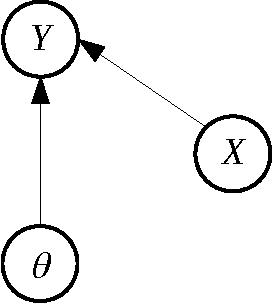
\includegraphics[width=.25\textwidth]{generative.pdf}\label{fig:generative}}
\hspace*{.2\textwidth}
\subfigure[Discriminative model]{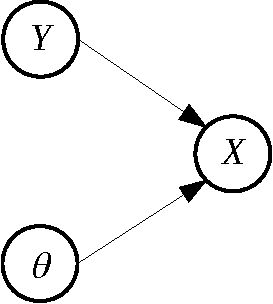
\includegraphics[width=.25\textwidth]{discriminative.pdf}\label{fig:discriminative}}
\caption{Bayesian networks representing generative and discriminative models, where $X$, $Y$ and $\theta$ respectively denote the variable of interest, the data, and the model parameters. Note the marginal independence of~$Y$ and~$\theta$ in the discriminative model.}
\label{fig:graph_comparison}
\end{center}
\end{figure}

Composite likelihood (CL, see \cite{Varin-11} and the references therein) is a semi-generative approach to statistical inference that extends the familiar notion of likelihood without requiring a full generative model. The key idea is to model an arbitrary set of low-dimensional features separately and then combine them, instead of modeling the data distribution as a whole. This may be viewed as a {\em divide and conquer} method to approximate the true but intractable likelihood. While maximum CL does not inherit the general property of maximum likelihood to yield an asymptotically minimum-variance estimator, it is consistent under mild conditions \cite{Xu-11} and may offer an excellent trade-off between computational and statistical efficiency in practice. 

In this note, CL is interpreted as a probabilistic opinion pool of ``agents'' making use of different pieces of information, or clues, extracted from the input data. Each agent acts as an isolated generative model-based statistician and expresses an opinion based on a single clue in the form of a likelihood function of the hidden variables. The agent opinions are then aggregated into a probability distribution on the hidden variables analogous to a Bayesian posterior.

We further argue that a particular log-linear opinion pool yields the best possible predictive distribution in the sense of maximum relative conditional entropy. This perspective entails a method to optimize the weights of the different agents from training data as in a typical discriminative learning scenario. 

%Something for true statisticians. Maybe we could clarify that we use the term ``Bayesian'' in the sense of ``empirical Bayesian'', implying that the parameters $\theta$ are to be estimated somehow contrary to a ``full Bayesian'' approach where they would be integrated out at inference time.


\section{Composite likelihood as opinion pooling}
\label{sec:pool}

Let $Y$ an observable multivariate random variable with sampling distribution $p(y|x)$ conditional on some unobserved variable of interest, $X\in{\cal X}$, where ${\cal X}$ is a known set. Given an experimental outcome $y$, the likelihood is the sampling distribution evaluated at $y$, seen as a function of $x$:
$$
L(x) = p(y|x)
.
$$

This requires a plausible generative model which, for complex data, may be out of reach or involve too many parameters to be estimated. A natural workaround known as {\em data reduction} is to extract some lower-dimensional representation $z=f(y)$, where $f$ is a many-to-one mapping, and consider the potentially more convenient likelihood function:
$$
\ell(x) = p(z|x)
.
$$

Substituting $L(x)$ with $\ell(x)$ boils down to restricting the sample space, thereby  ``delegating'' statistical inference to an ``agent'' provided with partial information. While it is valid for such an agent observing~$z$ only to consider $\ell(x)$ as the likelihood function of the problem, the drawback is that $\ell(x)$ might yield too vague a prediction of~$X$ due to the information loss incurred by data reduction. To make the trick statistically more efficient, we may extract several features, $z_i=f_i(y)$ for $i=1,2,\ldots,n$, and try to combine the likelihood functions $\ell_i(x) = p(z_i|x)$ that they elicit.

If we see the likelihoods as posterior distributions corresponding to uniform priors, this is a classical problem of probabilistic opinion aggregation from possibly redundant sources, for which several methods exist in the literature \cite{Tarantola-82,Genest-86,Garg-04,Allard-12}. We will show in Section~\ref{sec:maxent} that one that is particularly well-suited to our case is the {\em log-linear opinion pool}: 
\begin{equation}
\label{eq:log_pool}
p_\lambda(x|y) = \frac{1}{z_\lambda(y)} \pi(x) \prod_{i=1}^n p(z_i|x)^{\lambda_i},
\end{equation} 
where $\pi(x)$ is some reference distribution or prior, and $\lambda=(\lambda_1,\ldots,\lambda_n)$ is a vector of weights so that the normalizing factor:
$$
z_\lambda(y) = \int \pi(x) \prod_{i=1}^n p(z_i|x)^{\lambda_i} dx
$$
is finite, which holds whenever $\lambda\succeq 0$, {\em i.e.} all weights are positive, assuming that the agent opinions are always upper bounded. Negative weights should be ruled out as the existence condition $z_\lambda(y)<\infty$ would then depend on the particular opinions expressed by the agents. Also note that, while it is possible to have the weights depend on~$y$, there is a strong rational for constant weights as we shall see in the sequel. 

%Strictly positive weights guarantee the so-called 0/1 forcing property, that is, if an hypothesis~$x$ has zero likelihood according to at least one agent, then its consensus probability vanishes too.

% Not clear yet as to what a negative weight could mean!

The log-linear pool~(\ref{eq:log_pool}) bears a striking similarity to Bayes rule, yielding the form: $p_\lambda(x|y)\propto \pi(x) L^c_\lambda(x)$, where the quantity:
\begin{equation}
\label{eq:comp_lik}
L^c_\lambda(x) \equiv \prod_{i=1}^n \ell_i (x)^{\lambda_i}
\end{equation} 
plays the same role as a traditional likelihood function. This expression happens to be known in statistics as a {\em marginal composite likelihood} \cite{Varin-11}. See Appendix~\ref{sec:conditional} for the slightly more general form called {\em conditional composite likelihood}, which can be derived in the same way.

From~(\ref{eq:comp_lik}), we see that CL shares a convenient factorized form with the likelihood derived under the assumption of mutual feature independence, usually referred to as {\em na\"ive Bayes} or {\em simple Bayes} in the machine learning literature, which corresponds to the special case of unitary weights, $\lambda_1=\ldots=\lambda_n= 1$. The clear computational advantage of CL over the true likelihood is that it only requires to evaluate the marginal feature distributions rather than the joint distribution of all features.


\section{Tuning composite likelihood weights}

When the features can be considered exchangeable, it is natural to choose uniform CL weights. The CL is then a scaled version of the na\"ive Bayes likelihood, the common weight value being irrelevant to the maximum CL estimator (MCLE). The weight may be tuned so as to best adjust the pseudo posterior variance matrix to the asymptotic variance matrix of the MCLE \cite{Pauli-11}, or via a close-in-spirit curvature adjustment \cite{Ribatet-12}, in attempts to match the frequentist and composite Bayesian notions of uncertainty.

Ignoring such a goal, another frequent recommandation for CL weights is to sum up to one. This can be motivated in various ways. It turns out that the only pooling operator that does not explicitly depend on~$x$ and preserves {\em external Bayesianity} is the log-linear opinion pool with unit sum weights \cite{Genest-86b}. External Bayesianity essentially means that it should not matter whether the prior is incorporated before or after pooling, provided that all agents agree on the same prior. Another appealing property of log-linear pooling with unit sum weights is to minimize the average Kullback-Leibler (KL) divergence to the agent opinions \cite{Garg-04}. A maximum relative entropy property is also given in \cite{Wang-14}, Theorem~3.

Unit sum weights, however, correspond to the extreme situation where the features are assumed to be maximally redundant, but is clearly ineffective for independent or weakly correlated features, which require weights close to one for the CL to closely approximate the true likelihood. In this case, the CL may be much flatter than it should, leading to severly overestimated credibility sets.

{\color{red} Why is it important to fine-tune the weights?}
We therefore need a method to tune weights that can automatically adjust to the level of statistical dependence beween features.

%Instead, redundancy between agents is assumed by default, and is effectively encoded by the unit sum constraint on weights\footnote{Nevertheless, features which are {\em known} to be mutually independent can be merged into a single feature. This results in increasing their weights in the log-linear pool.}.

\section{Maxent composite likelihood}
\label{sec:maxent}

We can derive composite likelihood from the conditional maximum entropy principle \cite{BergerA-96}. It comes with a method of tuning weights, hence a particular composite likelihood function that we call maxent composite likelihood (MCL).

A cheap MaxEnt argument was already given by \cite{Wang-14}  (standard, non-conditional MaxEnt at fixed $y$, hence just an existence result but no feasible weight tuning).

What we do here is maximum {\em conditional} entropy. It's slightly more complex than a simple $I$-projection. The search space is a set of predictive distributions compatible with mean log-likelihood contraints. If I know the generative distribution, I know the expected log-likelihood.

We work with inequality constraints to force $\lambda\geq 0$:
$$
E[\log p(z_i|x)] \geq c_i \equiv \int \pi(x)p(z_i|x) \log p(z_i|x) dx dy
$$

What does the constraint mean? It means that a model is admissible if it compresses the data at least as well as all my agents. So we are not assuming that the generative models are {\em true}. We only assume that they are useful to compress the (reduced) data. Connection to MDL. 

Why not using the feature-based posteriors or Bayes factors rather than the likelihoods? It's a possibility (perhaps a connection here with Gr\"unwald's luckiness). A justification for not doing it is that the coordinator should discard the priors used by the agents. The constraints are not purely evidence-based since the moments depend on the coordinator's prior but it is arguable a mess of priors wouldn't be good.

Intuition behind weights: Lagrange multipliers to enforce a constraint... Notion of feature relevance. But does $\lambda_1>\lambda_2$ imply that $z_1$ is more relevant than $z_2$? 

The derivation assumed the marginal distribution of the data $h(y)$ to be known. In practice, it is estimated by the empirical distribution just like the moments are estimated.

Game theoretic interpretation \cite{Grunwald-04}.

The dual function boils down to the famous cross-entropy.

Single feature case ($y=z$): the maxent solution has the form $p(x|y)\propto\pi(x)p(y|x)^\lambda$. We expect to have $\lambda=1$ but it's not necessarily the case. It is if $h(y)=\int\pi(x)p(y|x)dx$ because then $h(y)p(x|y)=\pi(x)p(y|x)$ so the constraint is verified (and active). This also tells us that the data marginal should be consistent with the prior on labels for this much expected consistency property to hold. So, either weight datapoints so as to match a desired prior (e.g., uniform) or take the empirical distribution of labels as the ``prior''. 

Which brings another question: in this case, the (unique) weight is insensitive to the prior -- is it true in general? The answer is no. The weights generally depend on the prior. Hence the maxent composite likelihood is prior-dependent. This is an important conceptual difference with the classical notion of likelihood.

\section{Super composite likelihood}
\label{sec:super}

When chosen for computational simplicity, clues may not only convey limited information at individual level: their informativeness may also be very much hypothesis-dependent. Consider, for instance, diagnosing a disease from a routine medical checkup. Body temperature may point to a bacterial infection by comparison with normality, but would not help detecting a non-infectious cardiovascular disease -- and conversely for, say, blood pressure.

This motivates a more general setting where clues can be weighted differently depending on hypotheses.

What happens if we use mean-values constraints conditional on $x$ instead of jointly averaged over $x$ and $y$? This boils down to picking functions of the form:
$$
\chi(x-a)\ell_i(x,y)
$$

The answer is that the maxent solution has the form:
$$
p_\lambda(x|y) = \pi(x) \prod_i p(z_i|x)^{\lambda_i(x)}
$$

In other words, the weights become dependent on the variable of interest. This is the super composite likelihood idea.


\section{Composite EM algorithm for unsupervised learning}
\label{sec:gem}

In a nutshell: alternate unsupervised learning of partial model parameters ($M$-step) and re-estimation of label posteriors via maxent ($E$-step). 

$M$-step: given a posterior estimate $q(x|y)$, do just as if the features were independent and solve: 
$$
\max_\theta
\int \sum_i h(y)q(x|y) \log p_\theta(z_i,x) dx dy
$$

Note we can estimate cross-feature parameters such as class proportions.

Surrogate $E$-step: given generative parameters, recompute the moment constraints and update $q(x|y)$ according to the conditional maxent principle:
$$
\min_q
\int h(y)q(x|y) \log \frac{q(x|y)}{\pi(x)} dx dy
$$
s.t.
$$
\int h(y)q(x|y)\log p_\theta(z_i|x) dx dy \geq \int \pi(x)p_\theta(z_i|x)\log p_\theta(z_i|x) dx dy
$$

However, there is an important issue: how is $h(y)$ defined in both the $M$- and $E$-steps? In supervised context, $h(x,y)$ can be defined beforehand as the prior-corrected empirical distribution:
$$
h(x,y) = \pi(x) \frac{h_0(x,y)}{h_0(x)},
$$
where $h_0(x,y)$ is the raw empirical distribution. In unsupervised context, the best we can do is to replace $h_0(x,y)$ with $h_0(y)q(x|y)$, implying that the empirical distribution of $y$ is reweighted according to:
$$
h(y) = \sum_i w_i\delta(y-y_i),
\qquad
w_i = \int \pi(x)\frac{q(x|y_i)}{\sum_j q(x|y_j)} dx,
$$
which needs to be done each time $q(x|y)$ is updated, that is, after each $E$-step.

The other option is to keep $h(y)$ constant throughout the iterations but adapt $\pi(x)$ as the marginal distribution of labels learned in the $M$-step. In this case, it's no longer a ``prior''. 

Are we minimizing a unique functional as in the variational EM algorithm? Possibly not. We may see this generalization as a two-player game. One player tries to predict several data features independently. The other player tries to predict labels. Together, they find patterns (clusters) in unlabeled data. Does the more general version converge? Does the game have a value? And so on.

In the case of a single feature, is this the well-known EM? The $M$-step is clearly the same, what about the $E$-step? It is the same if $h(y)p_\theta(x|y)=p_\theta(y|x)\pi(x)$. However, this condition won't hold if $h(y)$ is an empirical distribution... In this special case, the ``E player'' could use the data distribution model produced by the ``M player'' instead of the empirical one but, more generally, there is no data distribution model so he has to stick to the empirical one.

The maxent is a surrogate for the $E$-step. It reflects the lack of a full model $p_\theta(x,y)$.

% Accounting here for Xi'An comment on xianblog.wordpress.com
% The sum of the powers is constrained to be equal to one, even though
% I do not understand why the dimensions of the projections play nog
% role in this constraint. Simplicity is advanced as an argument,
% which sounds rather weak…
%This simple constraint is implied by the external Bayesianity requirement: as it turns out, the only aggregation operator which is both externally Bayesian and independent from $x$ boils down to plugging a composite likelihood with unit sum weights into Bayes rule, hence extending the classical notion of likelihood in Bayesian analysis.


\section{Discussion}
\label{sec:discussion}

Deep learning is discriminative...

CL is a concept from computational statistics that has mainly been developed so far in a frequentist perspective as a surrogate for the maximum likelihood method. We have shown a deep connection between CL and probabilistic inference, thereby establishing CL as a class of discriminative models. Because CL is built from a set of marginal feature-specific generative distributions, it is in essence a two-step semi-generative, semi-discriminative learning approach. In the first, ``generative'' phase, the feature distributions are learned; in the second, ``discriminative'' phase, the feature weights are learned. This strategy can be thought of as a form of non-adaptive boosting.

%The first phase corresponds to the training of ``weak learners''. The second phase amounts to a form of boosting. 

A purely discriminative learning could be used instead but...
Why potentially more efficient than pure discriminative training: because generative training is always more efficient than discriminative training if models are comparable. So the key point is that ``we have less parameters in the discriminant phase". Good in small datasets. But also in asymptotic regime if the features are weakly or highly correlated (???).

Logistic regression / naive Bayes example. Under homoscedasticity (assuming that each feature has class-independent variance), CBI is equivalent to logistic regression -- because the predictive distribution family is the same. This is a case where BCI brings nothing. But consider heteroscedasticity, then BCI yields a quadratic classifier. Compared to a fully discriminative model, the number of parameters to learned in the discriminative phase is reduced by half.

The first training phase is easier if supervised but could be unsupervised too (using mixture models). How do we then deal with label switching issues? Can we safely assume conditional feature independence {\em in the generative training phase}? I believe so provided that the marginal distribution parameters are disjoint. It's obvious in the supervised learning scenario.

If unsupervised, the first learning phase could be compared with contrastive pre-training of RBMs \cite{Hinton-06,Fischer-14}, which also optimize parameters for generation of observable features. BCI is comparable with an RBM with a single output unit (which is just a generative model assuming conditionial feature independence). The key difference is that the RBM is a full generative model while BCI only deals with marginal models, hence relying on weaker assumptions. This won't change anything in the pre-training phase but RBMs have to deal with more parameters in the generative learning phase. In fully supervised context, RBM pre-training is pointless since all parameters learned in the first phase will be overwritten. In BCI, pre-training is crucial even in supervised context because the parameters learned in the discriminative phase (the feature weighs) describe a sub-manifold of the predictive distribution family.

Needs features. Not a representation learning method, but could be coupled why not.


%{\color{red} Moreover, while RBM parameters are typically refined in a supervised discriminative learning step, disjoint set of parameters for SCL. Dunno how to say that.} 

%In such context, SCL competes with classical discriminative models (logistic regression, Gaussian processes \cite{Rasmussen-06}, maximum entropy models \cite{BergerA-96}, etc.), and may compare more or less favorably in practice depending on the amount of training data. For relatively small training datasets, we may hope for more accurate inference using~SCL than using traditional discriminative models, extrapolating from the results of \cite{Ng-01} regarding the comparison between logistic regression and na\"ive Bayes classifiers.
%{\color{red}Ici, il manque la comparaison avec les RBMs qui ne sont pas (forcement) des modeles discriminatifs.}

%%, hence alleviating the need for heavily supervised model training

%In summary, CL has the potential to yield weakly supervised or unsupervised Bayesian-like inference procedures depending on the particular task at hand. This property reflects the encoding of statistical relationships between the data and {\em all} unknown parameters. CL thus appears as a trade-off between generative models, which are optimal for unsupervised learning but possibly intractable, and traditional discriminative models (logistic regression, Gaussian processes \cite{Rasmussen-06}, maximum entropy models \cite{BergerA-96}, etc.), which are inherently supervised. CL models are discriminative models assembled from atomic generative models and, from this point of view, may be considered as {\em semi-generative} models.

%CL may be considered as a {\em semi-generative} model: a discriminative model assembled from partial generative models.

%As a note of caution, we shall stress that the pre-determined weights assigned to the different associations between observed and unobserved values represent prior knowledge regarding the informativeness of clues. A poor choice of weights will inevitably result in a poor approximation to the ``true'' Bayesian posterior -- the posterior that would be obtained from a realistic generative model if it was tractable. In future work, we will investigate feature selection strategies to mitigate this problem.

% Improve the discussion on following aspects:
% ** Why is it compatible with unsupervised learning? Give more insight.
% ** Stress the contribution: class-specific weighting.
% * Pivotality argument.
% * Bayes is a special case of composite Bayes.

{\color{red}Product of fucking experts \cite{Hinton-02}. Log-linear pool to build a generative model (assuming in fact independence between experts). Better seen as a ``log-mixture model''. Sounds like each expert is associated with a class, so it's the same as a RBM. Contrastive learning approximates ML parameter estimation. The experts are learning jointly. It's just a generative model.}

{\color{red}Two-step training: generative phase then discriminative phase. Why is it cool?}

{\color{red}CBI is just a way to reweight Naive Bayes. What's the big deal? Can we really expect massively superior performance? Are we just talking about realistic credibility sets?}


\appendix

\section{Conditional composite likelihood}
\label{sec:conditional}

As a straightforward  extension of marginal CL, each feature-based likelihood may be conditioned by an additional ``independent'' feature $z^c_i = f^c_i(y)$ considered as a predictor of the ``dependent'' feature, $z_i=f_i(y)$, yielding the more general form:
\begin{equation}
\label{eq:cond_feat_lik}
\ell_i(x) = p(z_i|x,z^c_i).
\end{equation}

Conditioning may be useful if it is believed that $z^c_i$ alone is little or not informative about $x$, but can provide relevant information when considered jointly with $x$, as in the case of regression covariates, for instance. Equation~(\ref{eq:comp_lik}) then amounts to conditional CL \cite{Varin-11}, a more general form of CL also including Besag's historical {\em pseudo-likelihood} \cite{Besag-74} developed for image segmentation.


\section{Minimally discriminative model}

Let $\pi(x)$ some reference distribution that represents full
uncertainty about $X$. We wish to select the joint distribution
$p(x,y)$ that minimizes:
$$
I(p) = \int p(x,y) \log \frac{p(x|y)}{\pi(x)} dy,
$$ subject to feature mean-value constraints of the form:
$$
\int p(x,y) f(x,y) dx dy = \mu.
$$

There are two special cases of this problem in the literature.  On the
one hand, the {\em maximum entropy classifier} \cite{BergerA-96}
incorporates the constraint that $p(y)$ be known, however we will see
that this is not necessary. The {\em minimally informative likelihood}
method \cite{Yuan-99b,Yuan-99}, on the other hand, imposes that
$p(x)=\pi(x)$, hence assuming the form $p(x,y)=\pi(x)p(y|x)$. We won't
make such assumptions here and will consider the case where $\mu$ is
completely unknown.

The above problem is seen to be equivalent to minimizing the auxiliary
objective function:
$$
I(p,m) 
= \int p(x,y) \log \frac{p(x,y)}{\pi(x)m(y)} dxdy,
$$ over $p$ and $m$, subject to the same constraints on $p$. We note
that $I(p,m)=I(p)+D(p_y\|m)$, showing that the auxiliary function
essentially adds a penalty term to the actual objective in order to
force $p(y)$ close to $m(y)$.

Minimizing $I(p,m)$ along both $p$ and $m$ is basically a minimum KL
divergence problem between two convex distribution spaces, so there
must be a unique solution {\bf -- to be checked in
  \cite{Cover-91}}. It is similar to the rate-distortion problem in
information theory, which may be solved by alternate minimization,
yielding a Blahut-Arimoto algorithm.
\begin{itemize}
\item {\em Let's call it A-step}. Optimize $p(x,y)$ at fixed $m$
  s.t. constraint:
$$
\exists \lambda, \qquad
p_{\lambda,m}(x,y) = \frac{1}{Z(\lambda, m)} \pi(x) m(y) e^{-\lambda^\top t(x,y)}
$$
The actual $\lambda$ is found my maximizing the dual function
$\psi(\lambda,m)$, see below.
\item {\em Let's call it B-step}. Optimize $m(y)$ at fixed $p(x,y)$:
$$
m(y) = \int p(x,y) dx
$$
\end{itemize}

Upon convergence, the algorithm outputs both joint and marginal
distributions $p_{\star}(x,y)$ and $m_{\star}(y)$ that both depend on
$\mu$. By construction, we have that $p_{\star}(y) = m_{\star}(y)$,
therefore $p_\star(x|y)=p_{\star}(x,y)/m_{\star}(y)$.


\section{Comparison with maximum entropy classifier}

Lagrangian...
$$
{\cal L}(p,m,\lambda)
= 
\int p(x,y) \log \frac{p(x,y)}{\pi(x)m(y)} dxdy
+
\lambda^\top \left( 
\int p(x,y) f(x,y) dydy - \mu 
\right)
$$ where $\lambda$ represents a vector-valued Lagrange multiplier. At
fixed $m$, the solution has the form:
$$
p_{\lambda,m}(x,y) = \frac{1}{Z(\lambda,m)}
\pi(x) m(y) e^{-\lambda^\top f(x,y)} 
$$

Note that this implies that the conditional distribution is
independent of $m$ once $\lambda$ is determined,
$$
p_\lambda(x|y) = \frac{1}{z(\lambda,y)} \pi(x) e^{-\lambda^\top f(x,y)} 
$$

Also, the marginal is a modulation of $m(y)$:
$$
p_{\lambda,m}(y) = \frac{z(\lambda,y)}{Z(\lambda,m)} m(y)
$$

Dual function at fixed $m$:
$$
\psi(\lambda,m) 
\equiv \min_p {\cal L}(p,m,\lambda)
= 
- \log Z(\lambda,m) - \lambda^\top \mu
.
$$ 

An alternative expression is:
$$
\psi(\lambda, m)
= 
\int h(x,y) 
\log \frac{p_{\lambda,m}(x,y)}{\pi(x)m(y)} dxdy,
$$ where $h(x,y)$ is any distribution statisfying the
constraints. This shows that maximizing the dual function at fixed $m$
is essentially the same as minimizing the KL divergence
$D(h\|p_{\lambda,m})$ over $\lambda$, in other words fitting $h(x,y)$
by some distribution of the form $p_{\lambda,m}$. The fact that the
result does not depend on the particular $h(x,y)$ that is chosen, as
long as it satifies the constraint, is a general property of
exponential families.

We also have that the dual function associated with $I(p)$ reads:
\begin{eqnarray*}
\psi(\lambda) 
 & = & \min_m \psi(\lambda, m)\\
 & = & \int h(x,y) \log \frac{p_{\lambda}(x|y)}{\pi(x)} dxdy\\
 & = & -\int h(y) \log z(\lambda,y) dy - \lambda^\top \mu
\end{eqnarray*}

But, wait, that's exactly what we get in the maximum entropy
classifier! So, at the end of the day, we simply got an alternative
method to learn $\lambda$ in the maximum entropy classifier, i.e. the
Blahut-Arimoto algorithm as opposed to a brute-force maximization of
$\psi(\lambda)$. Both methods will converge to the same $\lambda$...

What it essentially means is that the optimal $\lambda$ is insensitive
to $m(y)$ as long as $m(y)$ is compliant in the sense that:
$$
m(y) = \int h(x,y) dx,
$$ for some distribution $h(x,y)$ statisfying the constraint. This is
true for the optimal $m_\star(y)$ output by the BA algorithm, but
also, for instance, for the empirical distribution of observations in
a training dataset used to estimate $\mu$, as proposed in
\cite{BergerA-96}. The only special property of $m_\star(y)$ is to
yield the full Bayesian model $p_\star(x,y)=p_\star(x|y)m_\star(y)$
that minimizes the discrimination information. We may not care too
much about that in practice since we will only use $p_\star(x|y)$. 

\section{Comparison with minimally informative likelihood}

Yuan \cite{Yuan-99} considered the situation where we add the
constraint that $p(x)=\pi(x)$ to the minimum discrimination inference
problem. Unknown is then the conditional distribution
$p(y|x)$. Lagrangian...
\begin{eqnarray*}
{\cal L}(p,m,\lambda)
 & = & 
\int \pi(x)p(y|x) \log \frac{p(y|x)}{m(y)} dxdy
+
\lambda^\top \left( 
\int \pi(x)p(y|x) f(x,y) dydy - \mu 
\right) \\
 & = & 
\int \pi(x)
\left( 
\int
p(y|x) \log \frac{p(y|x)}{m(y)} dy
+
\lambda^\top 
\int p(y|x) f(x,y) dy
- \mu 
\right)
dx 
\end{eqnarray*}

The derivative is given by,
$$
\frac{\partial\cal L}{\partial p(y|x)}
= 
\pi(x)\left[ 
1 + \log \frac{p(y|x)}{m(y)} 
+ \lambda^\top f(x,y)
\right],
$$
hence the optimal model at fixed $m$ has the form:
$$
p_{\lambda,m}(y|x) = \frac{1}{Z(\lambda,m,x)} m(y) e^{-\lambda^\top f(x,y)} 
$$

Note that the induced posterior distribution $p_{\lambda,m}(x|y)$ has
a different form from above unless the normalizing factor
$Z(\lambda,m,x)$ turns out independent from $x$. If this is not the
case, we no longer have the property that $p_{\lambda,m}(x|y)$ is
independent from $m$ given $\lambda$.

Dual function...
$$
\psi(\lambda,m) 
=
- \int \pi(x) \log Z(\lambda, m, x) dx
- \lambda^\top \mu
$$

Equivalently, for any distribution under the form $\pi(x)h(y|x)$ that
satisfies the moment constraint, we have:
$$
\psi(\lambda,m) 
=
\int \pi(x) h(y|x) \log \frac{p_{\lambda,m}(y|x)}{m(y)} dxdy
$$

Now, the real question is why should we constrain $p(x)$, which boils
down to a Bayesian prior in this context, to be the same as our
reference $\pi(x)$? It only makes sense if we want our inference to
stick to a generative modeling paradigm... but haven't we already
given up on that? Therefore, unless we find a good reason not to, we
won't impose the $p(x)=\pi(x)$ constraint, thereby allowing for a
discrepancy between the reference and the prior.


\section{Discriminative vs. semi-discriminative}

Let's go back to the equivalence we found between our approach and the
maximum entropy classifier (MCE) \cite{BergerA-96}. We have said that
the former is essentially a re-formulation of MCE.

But the re-formulation also conveys a generalization of MCE if,
instead of letting $m$ being an arbitrary distribution, we restrict
its search space to some set of acceptable reference
distributions. Would such a strategy be useful? 

Recall that the method selects the joint distribution that minimizes
discriminative information, as defined by $I(p)$:
$$
I(p) 
= \int p(x,y)\log\frac{p(x|y)}{\pi(x)} dxdy
= E_Y[D(p_{x|y}\|\pi)]
$$

The latter characterization reminds us that discriminative information
is defined in an average sense. The corresponding posterior $p(x|y)$
may not be conservative for some $y$, in particular those that are
unlikely under $p(y)$. It would be a problem if that's the case for
the particular data at hand. For that to happen rarely, the ideal
$p(y)$ would be the ``true'' marginal distribution of $Y$.

However, for vague mean value constraints, nothing may prevent the
optimal $m_\star(y)$ from departing significantly from that ideal
distribution. In fact, we can show that $m_\star(y)$ only has mass at
$y$ values that maximize $z(\lambda_\star,y)$, and is therefore likely
sparse. This is because $m_\star$ minimizes $\psi(\lambda_\star,m)$,
which is equivalent to maximizing $Z(\lambda_\star,m)$ and we have:
$$
Z(\lambda, m) = \int m(y) z(\lambda, y) dy.
$$

In other words, the solution to our problem may be singular! It does
not hurt since, as discussed above, one may alternatively fix $m(y)$
to some pre-defined distribution... but this, in practice, restricts
the method to supervised learning situations.

We may not face this issue with the MIL method, which further imposes
the prior on $X$, so all the information from the constraints goes
into specifying a possibly reasonable generative model.



\bibliographystyle{abbrv}
\bibliography{cvis,stat,alexis}

%%\input{draft.biblio}

\end{document}


\end{document}


\end{document}


\end{document}
